%--------------------
% Packages
% -------------------
\documentclass[11pt,a4paper]{article}
\usepackage{pdfpages}

\usepackage[utf8x]{inputenc}
\usepackage[T1]{fontenc}
%\usepackage{gentium}
\usepackage{mathptmx} % Use Times Font
\usepackage{amsmath} % For bmatrix environment


\usepackage[pdftex]{graphicx} % Required for including pictures
\usepackage[pdftex,linkcolor=black,pdfborder={0 0 0}]{hyperref} % Format links for pdf
\usepackage{calc} % To reset the counter in the document after title page
\usepackage{enumitem} % Includes lists

\frenchspacing % No double spacing between sentences
\linespread{1.2} % Set linespace
\usepackage[a4paper, lmargin=0.1666\paperwidth, rmargin=0.1666\paperwidth, tmargin=0.1111\paperheight, bmargin=0.1111\paperheight]{geometry} %margins
%\usepackage{parskip}

\usepackage[all]{nowidow} % Tries to remove widows
\usepackage[protrusion=true,expansion=true]{microtype} % Improves typography, load after fontpackage is selected

\usepackage{lipsum} % Used for inserting dummy 'Lorem ipsum' text into the template


%-----------------------
% Set pdf information and add title, fill in the fields
%-----------------------
\hypersetup{ 	
pdfsubject = {Sanjit Sarda's Implementation of DeePC for MAE 271D Final Project},
pdftitle = {MAE 271D Final Project: DeePC},
pdfauthor = {Sanjit Sarda}
}

%-----------------------
% Begin document
%-----------------------
\begin{document}

%-----------------------
% Title Section
%-----------------------
\begin{center}
    \Large\textbf{Simplified Implementation of DeePC} \\
    \normalsize
    MAE 271D \\
    Sanjit Sarda \\
    \today
\end{center}

\vspace{1em}
\hrule
\vspace{2em}

%-----------------------
% Main Content
%-----------------------

\section{Abstract}
Data-Enabled Predictive Control (DeePC) is a data-driven optimal control method that enables predictive control without requiring an explicit model of the system. DeePC exploits the behavioral system framework to learn the system dynamics without explicitly characterizing the system through system identification. In addition to discussing implementation notes and challenges, this project also shows how to speed up the compute of DeePC without loss of generality.


\section{Introduction}
% Deeper(haha) into DeePC, what why how

Model Predictive Control involves solving a finite-horizon optimization problem based on a predictive model of the system. This requires an accurate parametric model, which we can find through system identification, which can be difficult for many nonlinear systems, especially black boxes.

Data-Enabled Predictive Control (DeePC) solves this problem by offering a model-free framework. DeePC operates directly on measured input/output data, by leveraging the behavioral systems framework. The system is represented within an implicit model stored within Hankel matricies constructed from historical data. This representation effectively captures the system's behavior including non-linearities by capturing rolling window information from past and present data, allowing modeling without explicit system identification.

\section{Assumptions}
% System Dynamics & Model Used
% Constraints
% Disturbance
% Data collection, distribution, rationale etc
This implementation of DeePC in this report is based on a 2D double integrator system. The assumptions underlying the simulation and control setup are outlined below:

\subsection{System Dynamics}
The system is modeled as a continuous-time double integrator with the following state-space representation:
\[
\dot{x}(t) = A x(t) + B u(t), \qquad y(t) = C x(t)
\]
where the state vector \(x \in \mathbb{R}^4\) consists of position and velocity in two dimensions, and the control input \(u \in \mathbb{R}^2\) represents acceleration commands.
For a double integrator:

$$A = \begin{bmatrix}
\mathbf{0} & I_n \\
\mathbf{0} & \mathbf{0}
\end{bmatrix},
B = \begin{bmatrix}
\mathbf{0} \\
I_n
\end{bmatrix},
C = \begin{bmatrix}
I_n & \mathbf{0}
\end{bmatrix},
D = \mathbf{0}$$


The system is discretized using zero-order hold with a sampling period \(dt = 1.0\), resulting in discrete-time matrices \(A_d, B_d\).

\subsection{Constraints}
Box constraints are imposed on both the system state and inputs:
\begin{itemize}
    \item Position and velocity components of the state are constrained to \([-10, 10]\).
    \item Control inputs (accelerations) are constrained to \([-2, 2]\).
\end{itemize}

\subsection{Disturbance Model}
Additive Gaussian noise is injected to the output of the system at each time step to simulate measurement disturbances. The covariance matrix was selected to be
$$\sigma = \begin{bmatrix}
    0.1  & 0.05 \\
    0.05 & 0.04
\end{bmatrix}$$

And two means, $\mu$ were selected as $\mathbf{0}$ and $\mathbf{0.1}$ to test its performance on steady state error. 

\subsection{Data Collection}
Offline input/output data is collected by applying random inputs spanning the range of allowable inputs. For a Linear System, this was found to be sufficient information, since
a carefully designed persistently exciting input sequence.

Online Data Collection is collected by using an MPC to drive the system from a pre determined state to the desired initial state. This is designed to emulate online data collection in a real system, where the system will likely be manually controlled before allowing DeePC to autopilot and plan a trajectory.

\subsection{Simplifications}
To focus on DeePC's core mechanics, the following simplifications are made:
\begin{itemize}
    \item The full system state is observable and used directly for output. This includes position and velocity data
    \item The system structure (double integrator) is known but not exploited—DeePC operates entirely from data.
    \item The dynamics are linear and time-invariant.
    \item Offline data is collected disturbance free.
\end{itemize}


\section{Problem Formulation}
% Optimization Problem
% Horizon, Cost, Constraints
% State/Input Vectors
% Regularizations

DeePC very simply reformulates the optimal control problem by replacing the dynamics constraints with the implicit model constraints.

\subsection{Traditional MPC Formulation}
In MPC, given a discrete-time linear system:
\[
x_{k+1} = A x_k + B u_k, \quad y_k = C x_k
\]
the objective is to minimize a cost over a finite horizon \( N \), subject to dynamics and constraints:
\[
\min_{u, x} \sum_{k=0}^{N-1} \left( \|x_k - x_{\text{ref}}\|_Q^2 + \|u_k\|_R^2 \right)
\]
\[
\text{s.t.} \quad x_{k+1} = A x_k + B u_k,\quad u_k \in \mathcal{U},\quad x_k \in \mathcal{X}
\]

For this formulation, we are using the following Cost Parameters:
$$Q = \mathbf{I}, Qf=5\mathbf{I}, R=2\mathbf{I}$$

A Receding Horizon Control is used, with 8 simulation steps, and a max horizon length of 4. Once fewer than 4 simulation steps are left, the horizon length becomes the remaining number of simulation steps.


\subsection{DeePC Formulation}
DeePC bypasses the need for the matrices \(A, B, C\) by using Hankel matrices derived from previously collected input/output data. These matrices implicitly encode the system behavior:
\[
H_L(u) = \begin{bmatrix}
u_1 & u_2 & \cdots & u_{T-L+1} \\
\vdots & \vdots & \ddots & \vdots \\
u_L & u_{L+1} & \cdots & u_T
\end{bmatrix}
\]

The Hankel matrix is a function of offline data and L. L represents the maximum context length available, and T represents how much offline data is within any given $u$. Therefore collecting more offline data results in a larger Hankel Matrix, and increasing the desired context length also increases the size of the Hankel Matrix.

We can then split the Hankel matricies into past and future data, where the past data is correlated with the \textit{initial condition} context available to the controller, and the future data is correlected with the future of the controller.

Given:
\begin{itemize}
    \item \( T_{\text{ini}} \): length of initial trajectory,
    \item \( N \): prediction horizon,
    \item \( U_{\text{off}}, Y_{\text{off}} \): collected input/output data,
\end{itemize}
we construct the Hankel matrices:
\[
\begin{aligned}
\begin{bmatrix}
U_p \\
U_f
\end{bmatrix}
&= H_{T_{\text{ini}} + N}(U_{\text{off}}), \\
\begin{bmatrix}
Y_p \\
Y_f
\end{bmatrix}
&= H_{T_{\text{ini}} + N}(Y_{\text{off}})
\end{aligned}
\]
where \(U_p, Y_p\) capture the past data used to infer the system's current state, and \(U_f, Y_f\) are used for prediction.

The DeePC optimization problem is formulated as:
\[
\begin{aligned}
\min_{g, u, y, \sigma_y} &\quad \sum_{k=0}^{N-1} \|y_k - r_k\|_Q^2 + \|u_k\|_R^2 + \lambda_g \|g\|_1 + \lambda_y \|\sigma_y\|_1 \\
\text{s.t.} &\quad \begin{bmatrix} U_p \\ Y_p \\ U_f \\ Y_f \end{bmatrix} g = \begin{bmatrix} u_{\text{ini}} \\ y_{\text{ini}} + \sigma_y \\ u \\ y \end{bmatrix} \\
&\quad u_k \in \mathcal{U}, \quad y_k \in \mathcal{Y}
\end{aligned}
\]

Here, the implicit model is encoded within g.

For the sake of consistency and comparability, the same Cost parameters and Control Horizon is used here.

\subsection{Regularization}
The terms \( \lambda_g \|g\|_1 \) and \( \lambda_y \|\sigma_y\|_1 \) serve to regularize the optimization:
\begin{itemize}
    \item \( \lambda_g \) penalizes large weights in the implicit model.
    \item \( \lambda_y \) accounts for measurement noise in the initial output trajectory.
\end{itemize}

\section{Method}
This implementation was written in Python using NumPy and CVXPY.

\subsection{Simulation Framework}
The controlled system is a two-dimensional double integrator with four states: positions and velocities in the \(x\) and \(y\) axes. The system is modeled in continuous time and discretized using SciPy’s \texttt{cont2discrete} with a sampling period of 1.0s.

The simulation includes:
\begin{itemize}
    \item Gaussian noise injection
    \item Hard box constraints on states and inputs.
    \item Step-by-step simulation logic in a \texttt{DoubleIntegrator} class.
\end{itemize}

\subsection{Offline Data Collection Loop}
A specified amount of data, $T = 200$ is collected. As previously mentioned, since this was a Linear System it was found any random set of inputs was sufficient to reliably estimate the system behavior.

\subsection{Online Control Loop}
A rolling horizon DeePC controller was implemented using the following steps:
\begin{enumerate}
    \item After each time step, the most recent input/output data (length \(T_{\text{ini}}\)) is saved. 
    \item The DeePC optimization problem is solved using CVXPY.
    \item The first control input from the solution is applied to the system.
\end{enumerate}

\subsection{Testing}
Testing was performed by using an MPC to steer the system to a setpoint for online data collection and then using DeePC to steer the system to $\begin{bmatrix}
    0 & 0
\end{bmatrix}$

The following starting points were used:
\begin{enumerate}
    \item $\begin{bmatrix}0 & 0 & 0 & 0\end{bmatrix}$
    \item $\begin{bmatrix}0 & 0 & 0 & 5\end{bmatrix}$
    \item $\begin{bmatrix}7 & -6 & -5 & -0.5\end{bmatrix}$
    \item $\begin{bmatrix}-3 & 2 & 0.5 & 0\end{bmatrix}$
    \item $\begin{bmatrix}0 & 0 & -2.5 & -4\end{bmatrix}$
\end{enumerate}

\subsection{Interpretability}

There are two interesting ways to interpret DeePC.
\subsubsection{Visualizing the Hankel Matrix}
If you look at the Hankel matrix, you can see the diagonal structure in the matrix that shows it as a sliding window of data.
\begin{figure}
	\centering
	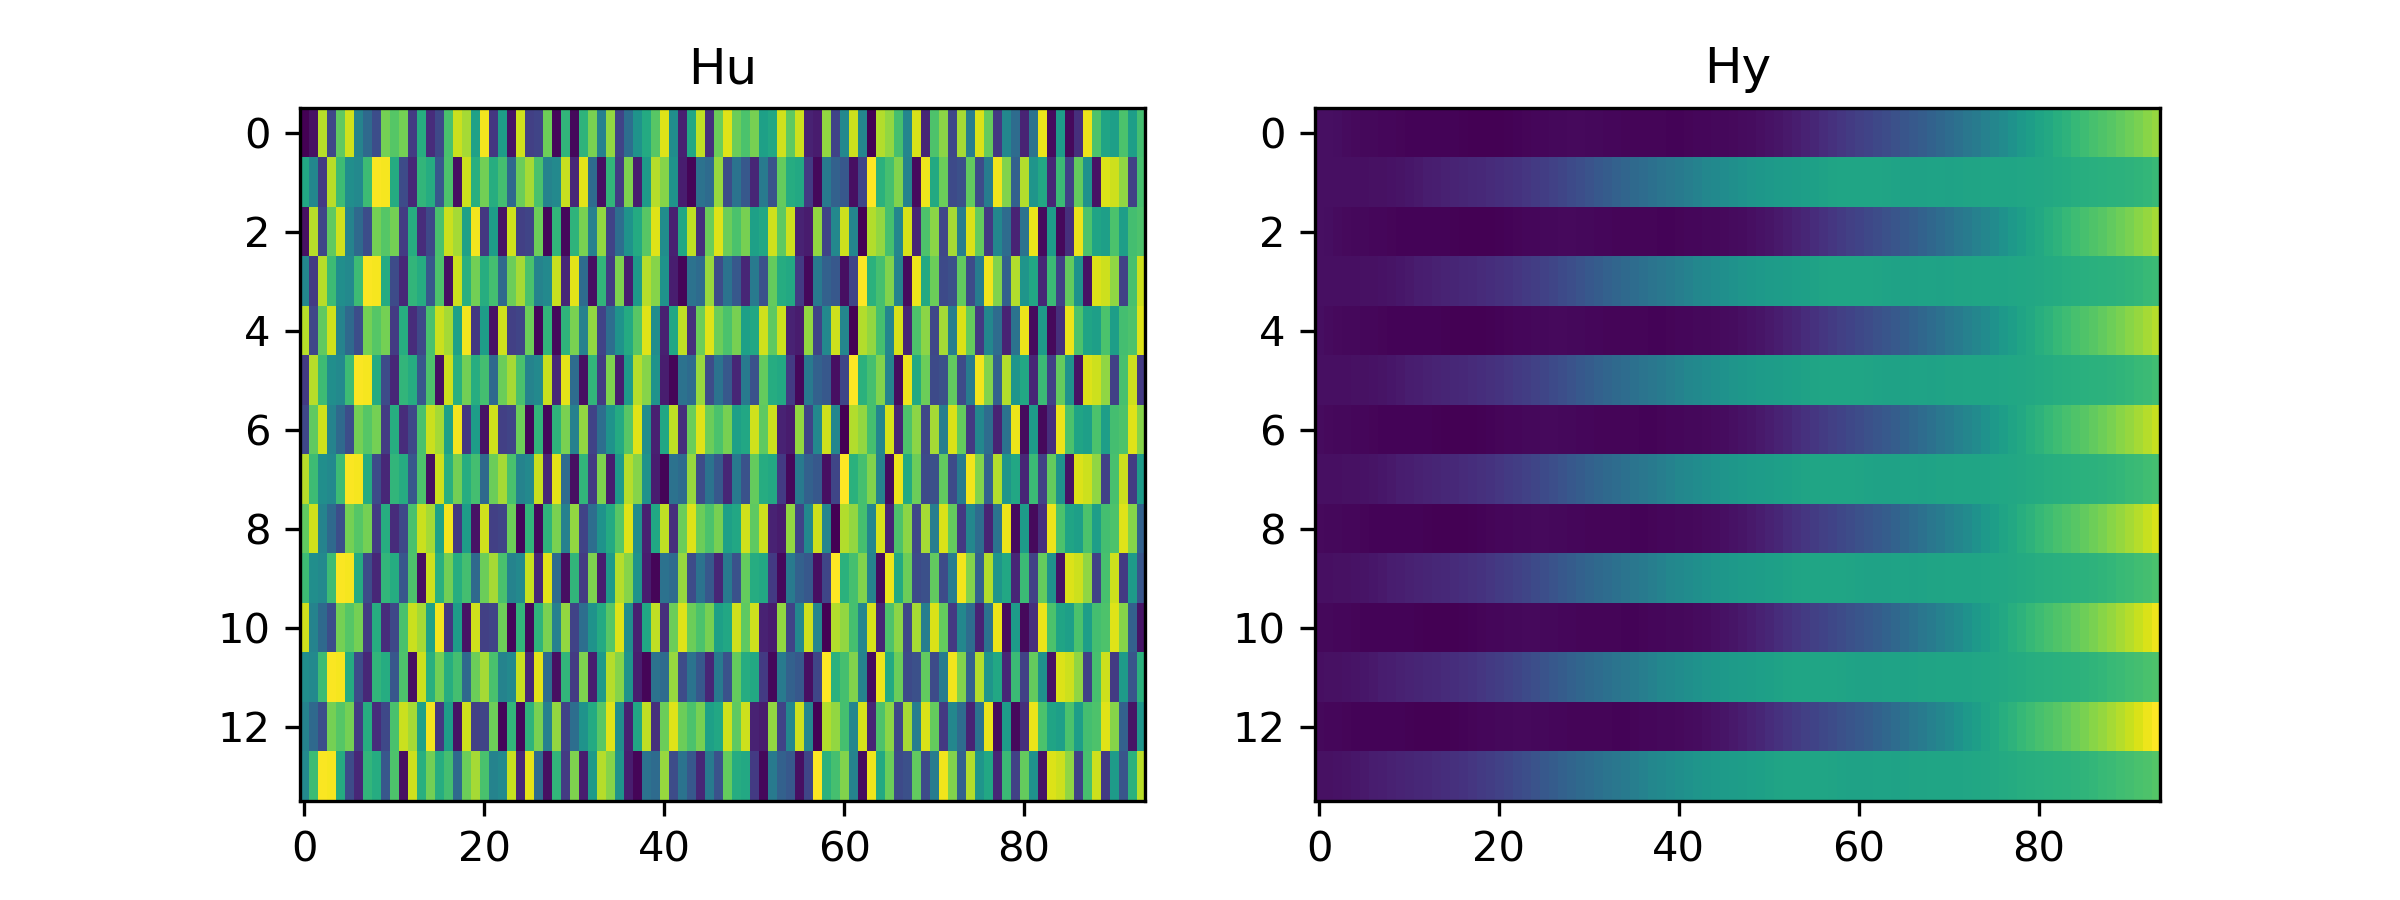
\includegraphics[width=0.85\linewidth]{./figures/deePC_hankel_matrices_imshow.png}
	\caption{Hankel Matrix of the Offline Data Collected}
	\label{fig:hankel-matrix}
\end{figure}

\subsubsection{System Identification}


To demonstrate System Identification using a Hankel Matrix, and why DeePC works, a useful demonstration is to extract the discretized $A_d$ and $B_d$ matricies from the offline data.

Since the Hankel Matrix is a sliding Window of data, we can say
$$X_f=A X_p +B U_p$$
$$\because x_{k+1}=Ax_k+Bu_k$$

So, $
\begin{bmatrix}
    A & B
\end{bmatrix}=
X_f
\begin{bmatrix}
    Xp \\
    U_p
\end{bmatrix}^{\dagger}
$

To run this with our offline data, and correctly collect the AB matricies, we need our output to be the whole state variable and the order to be 1, such that only past context is needed(no second derivatives in double integrator with pos and velocity state). Running this on the offline collected data, we get


Estimated A matrix:
$\begin{bmatrix}
    1 & -0 & 1 & 0 \\
    0 & 1 & 0 & 1 \\
    -0 & 0 & 1 & 0 \\
    -0 & 0 & -0 & 1
\end{bmatrix}$
Estimated B matrix:
$\begin{bmatrix}
    0.5 & -0 \\
    0 & 0.5 \\
    1 & 0 \\
    -0 & 1
\end{bmatrix}$

Which is exactly what we expect.

\section{Results}
First, we should look at the performance of an MPC controller on the system so that we have something to compare DeePC against.


\begin{figure}
    \centering
    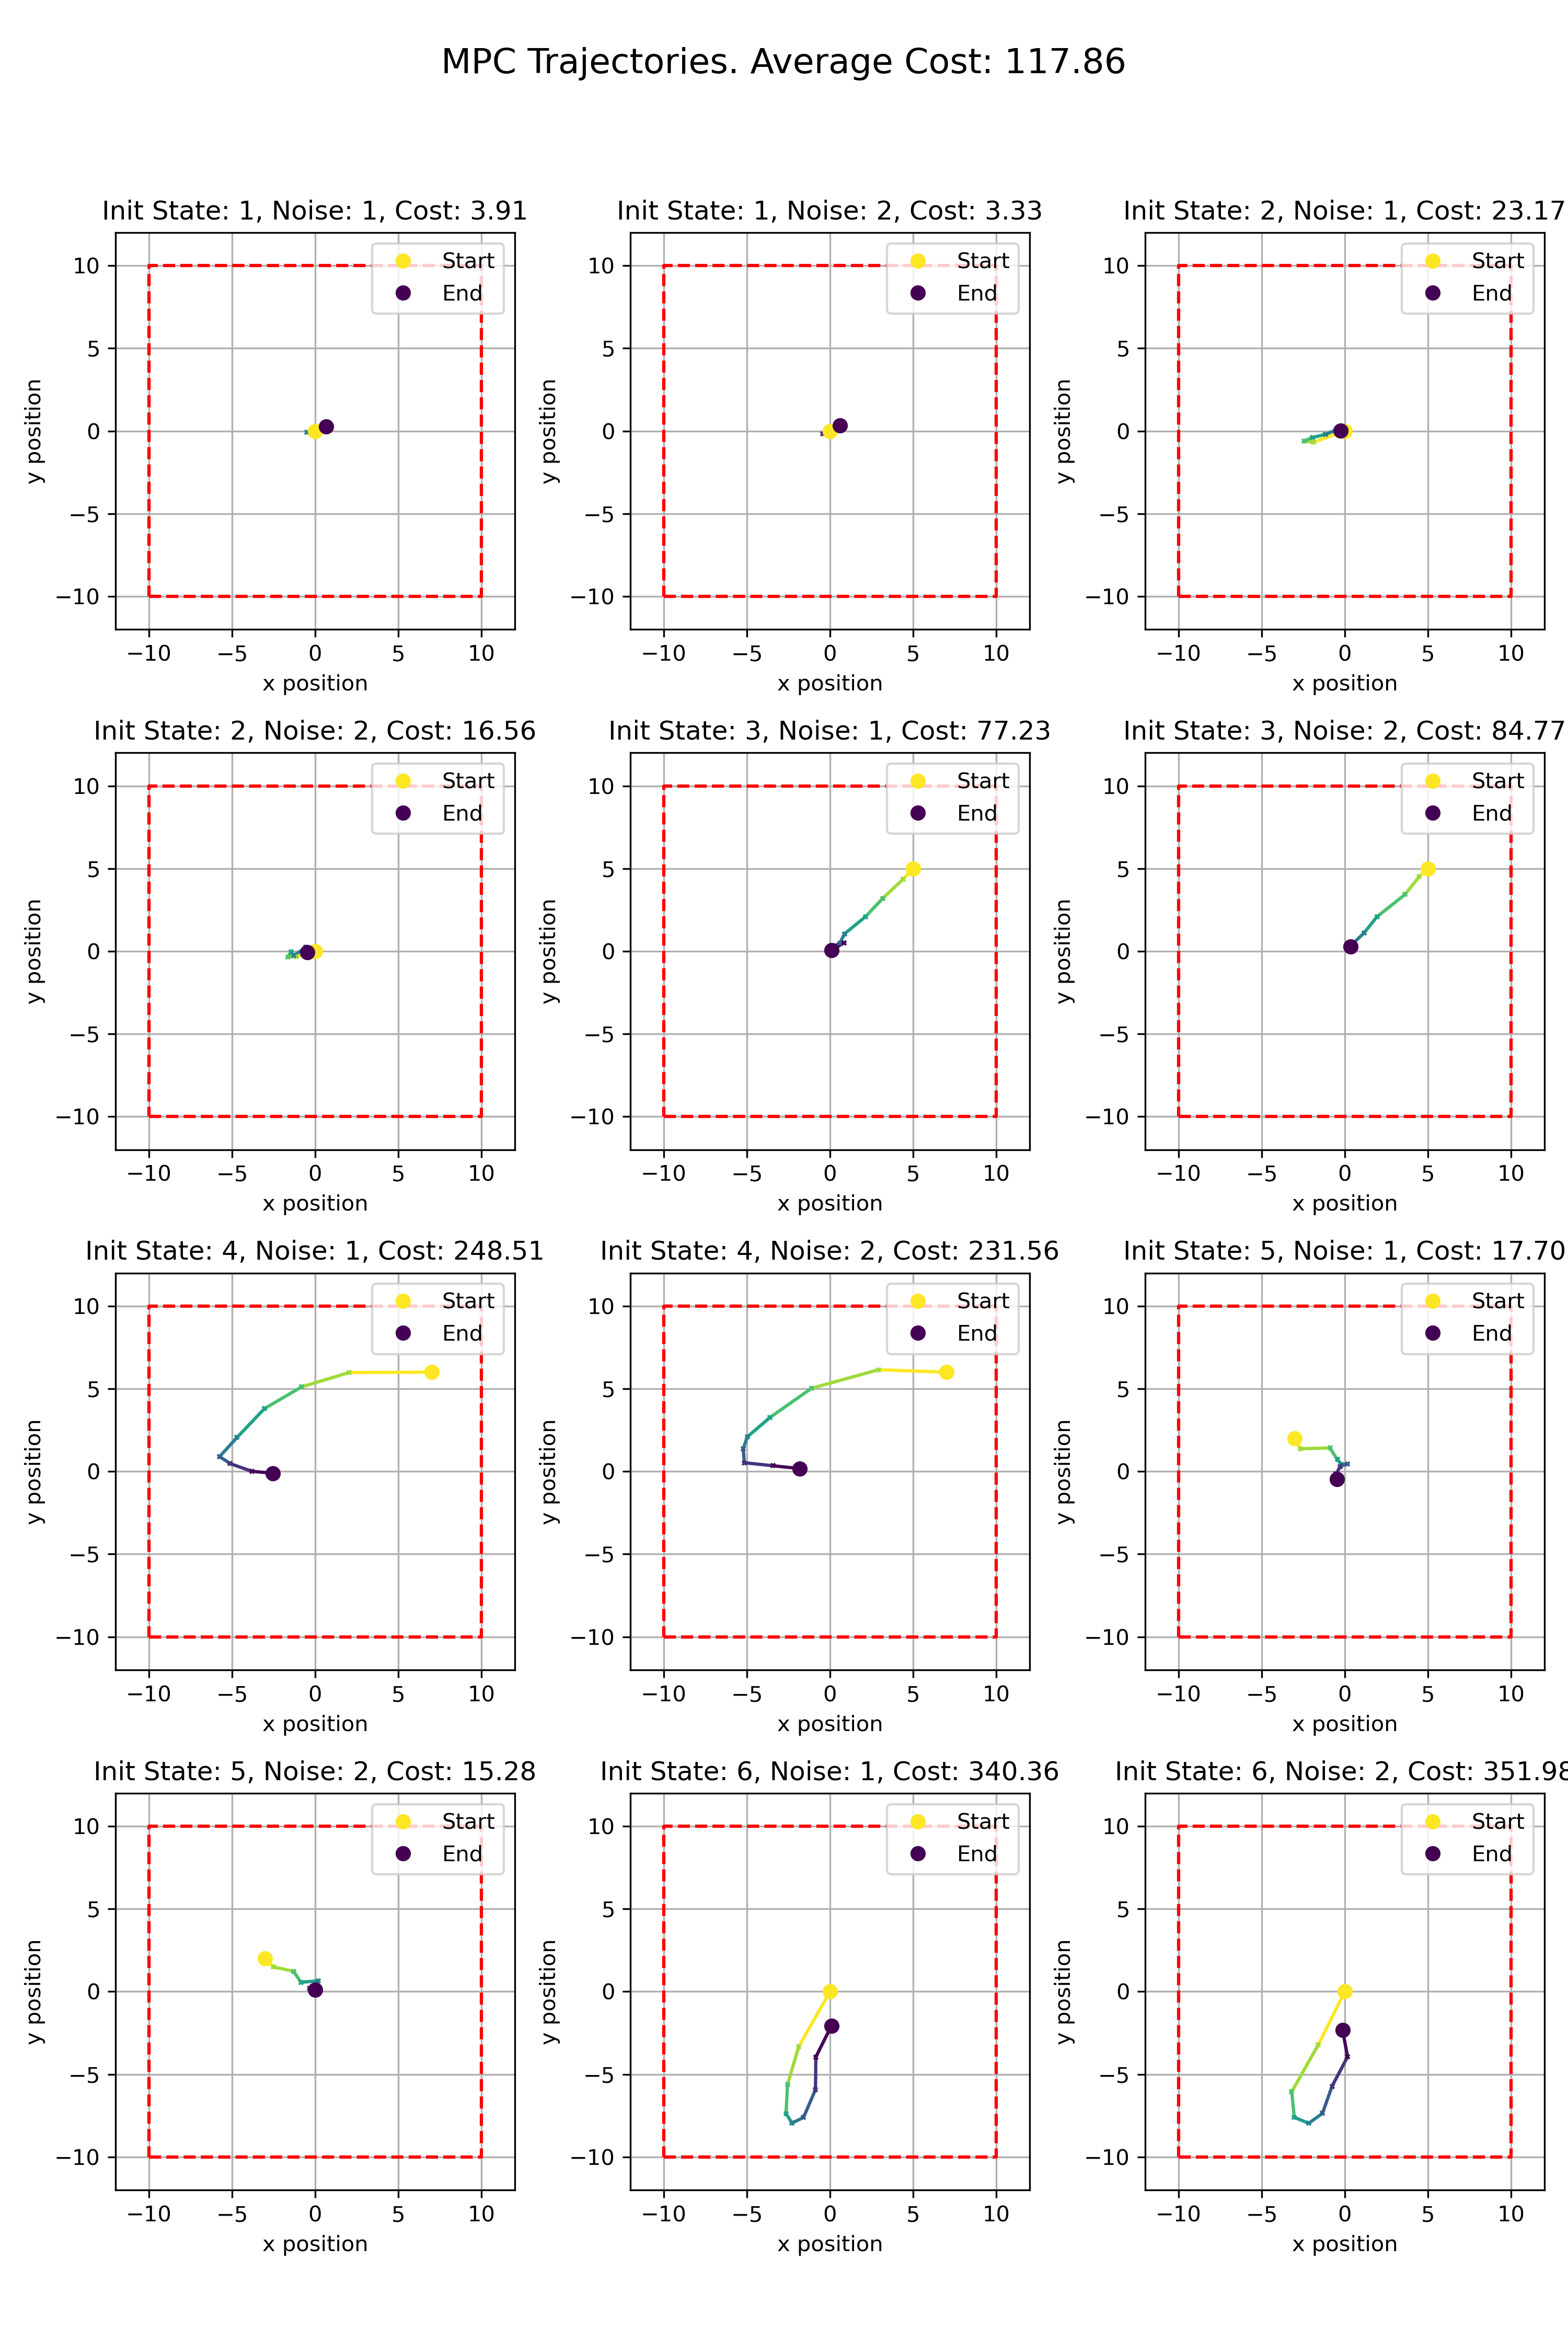
\includegraphics[width=0.85\linewidth]{./figures/mpc_trajectories.png}
    \caption{MPC performs fairly well, and optimizes over the the the entire state.}
    \label{fig:enter-label}
\end{figure}

These are the Hyperparameters to tune.
\begin{itemize}
    \item \textbf{Order Estimate}: This controls the "context" window for the implicit model to understand the current state of the system.
    \item \textbf{T}: Length of Offline samples collected.
    \item \( \mathbf{\lambda_g} \): Regulates the model size
    \item \( \mathbf{\lambda_y} \): Regulates the weight on the slack variable.
\end{itemize}


\subsection{Hyperparameter Testing}
Here are figures from Hyperparameter Testing with analysis


% Default
\begin{figure}
    \centering
    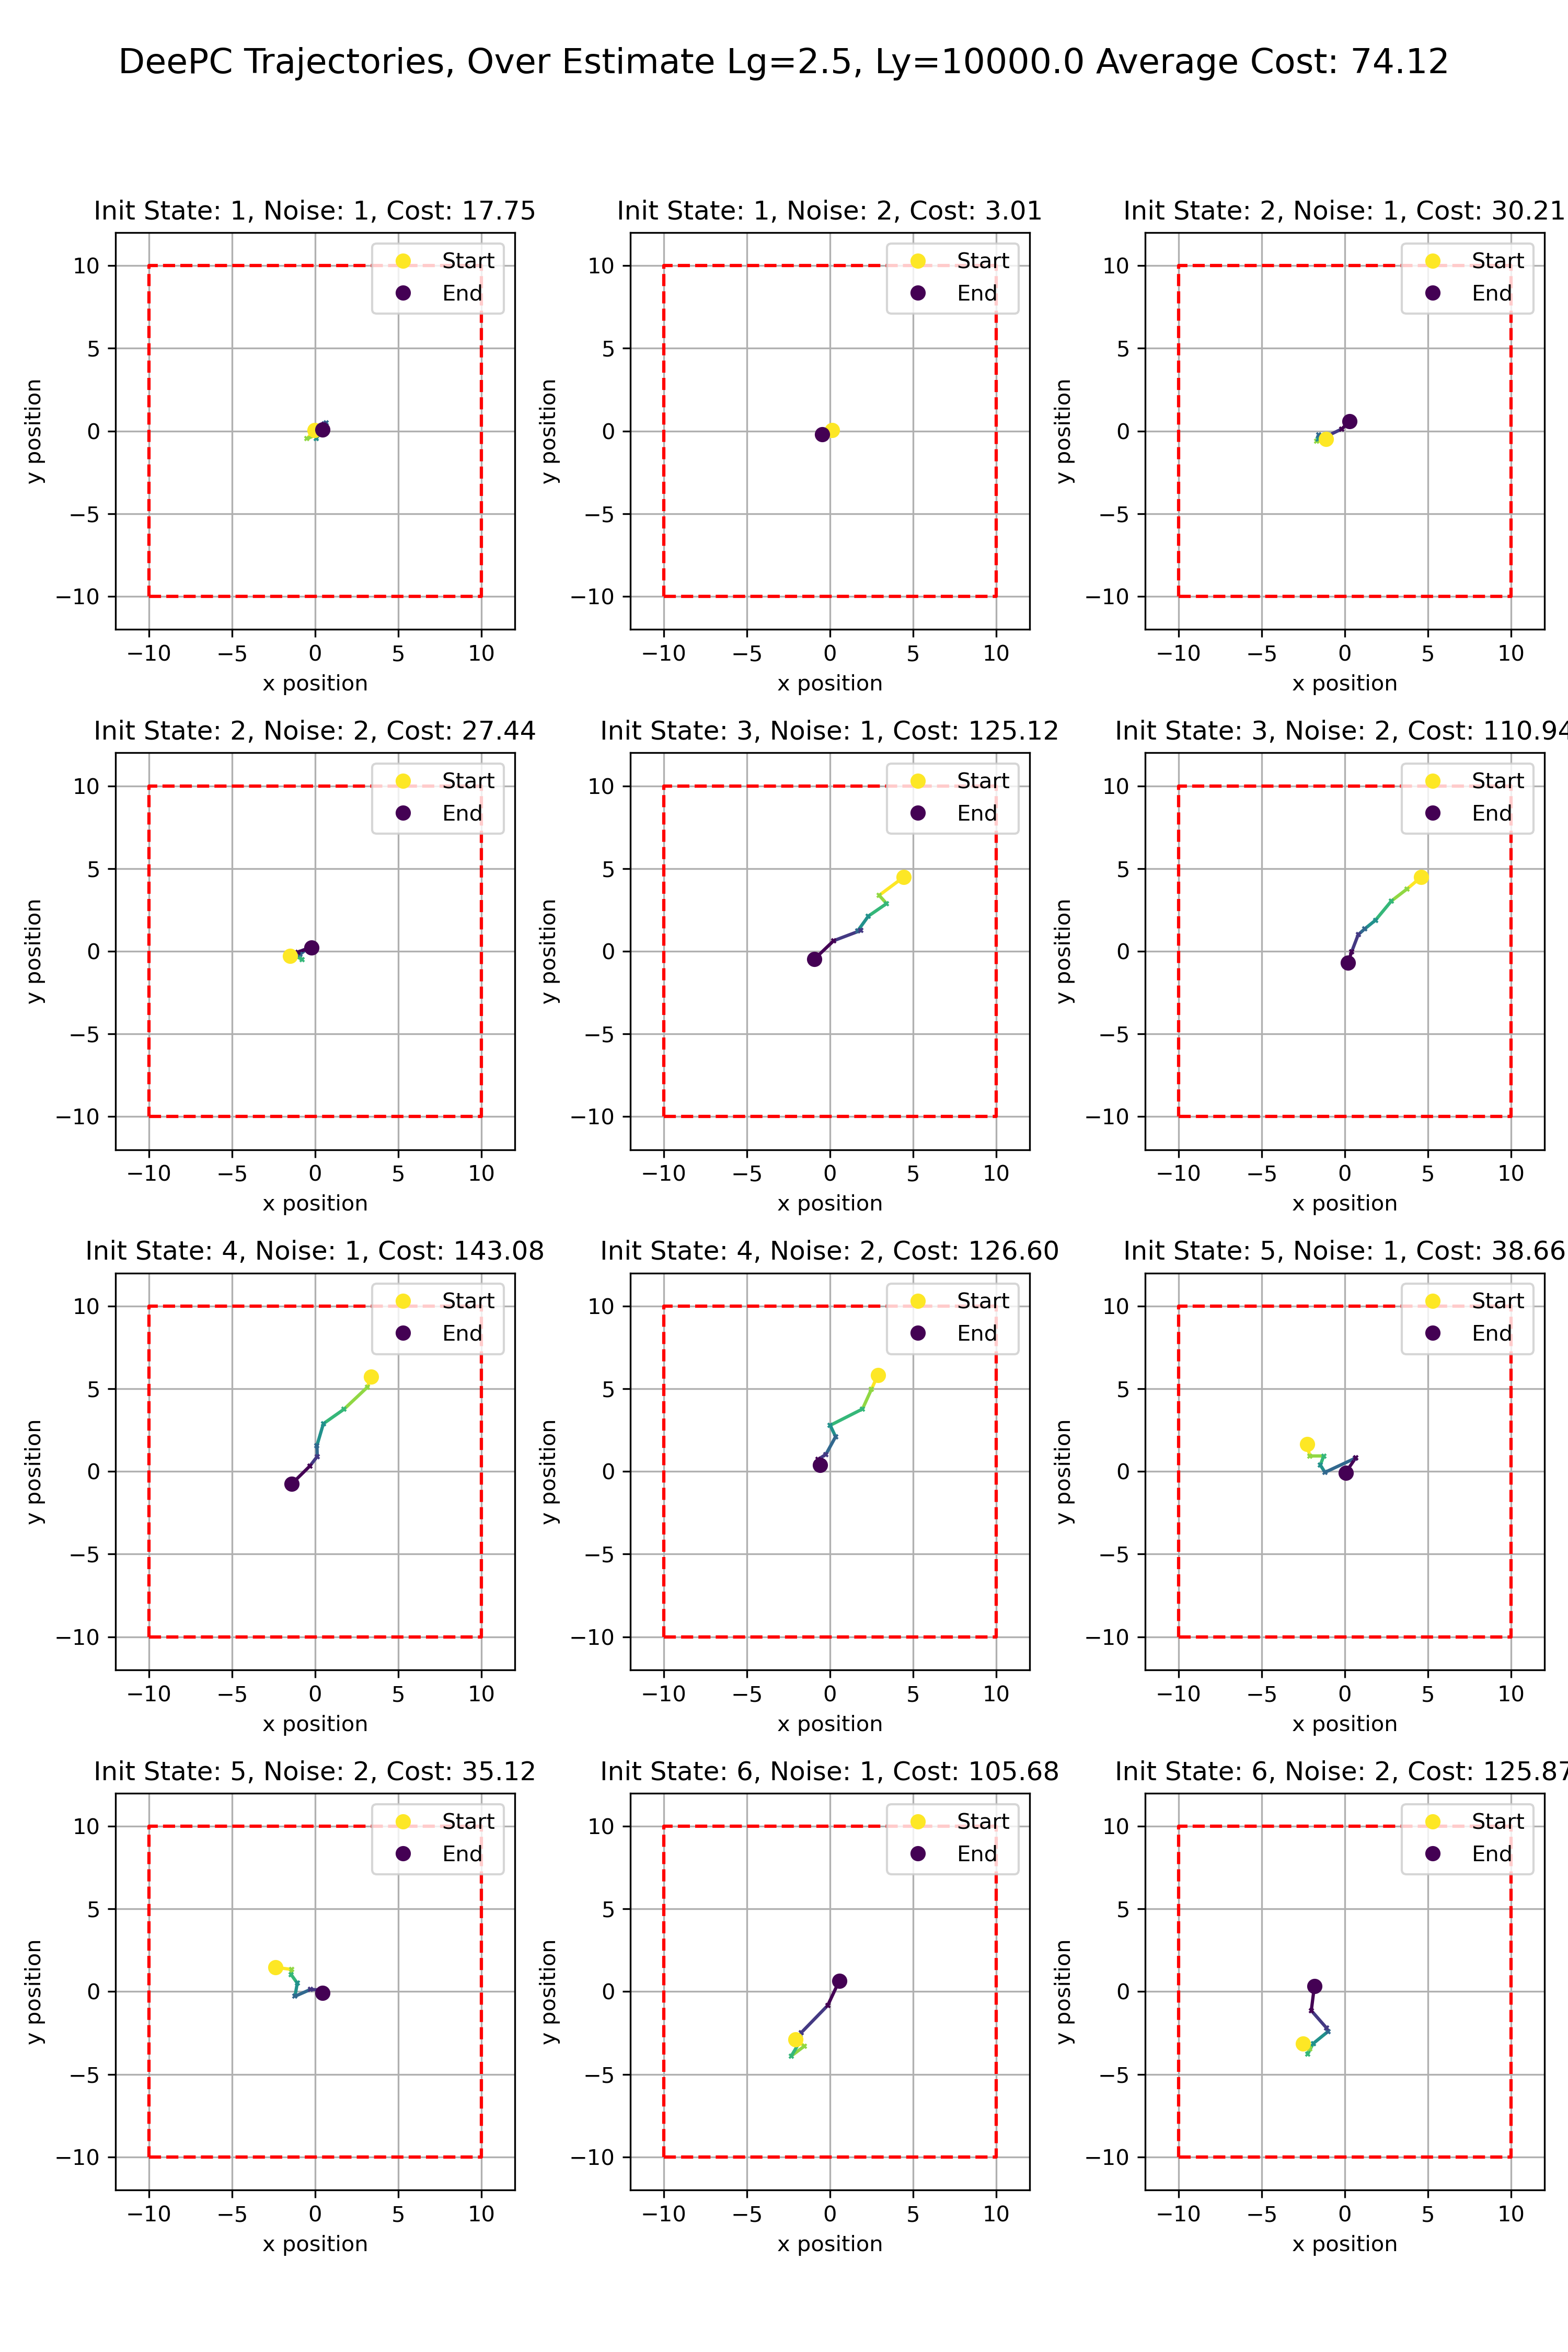
\includegraphics[width=0.85\linewidth]{./figures/DeePC_trajectories_2.5_10000.0.png}
    \caption{$\lambda_g=2.5, \lambda_y=1\mathrm{e}4, \text{order}=2, T=100$ Performs fairly well}
    \label{fig:enter-label}
\end{figure}

% Under Estimate Order
\begin{figure}
    \centering
    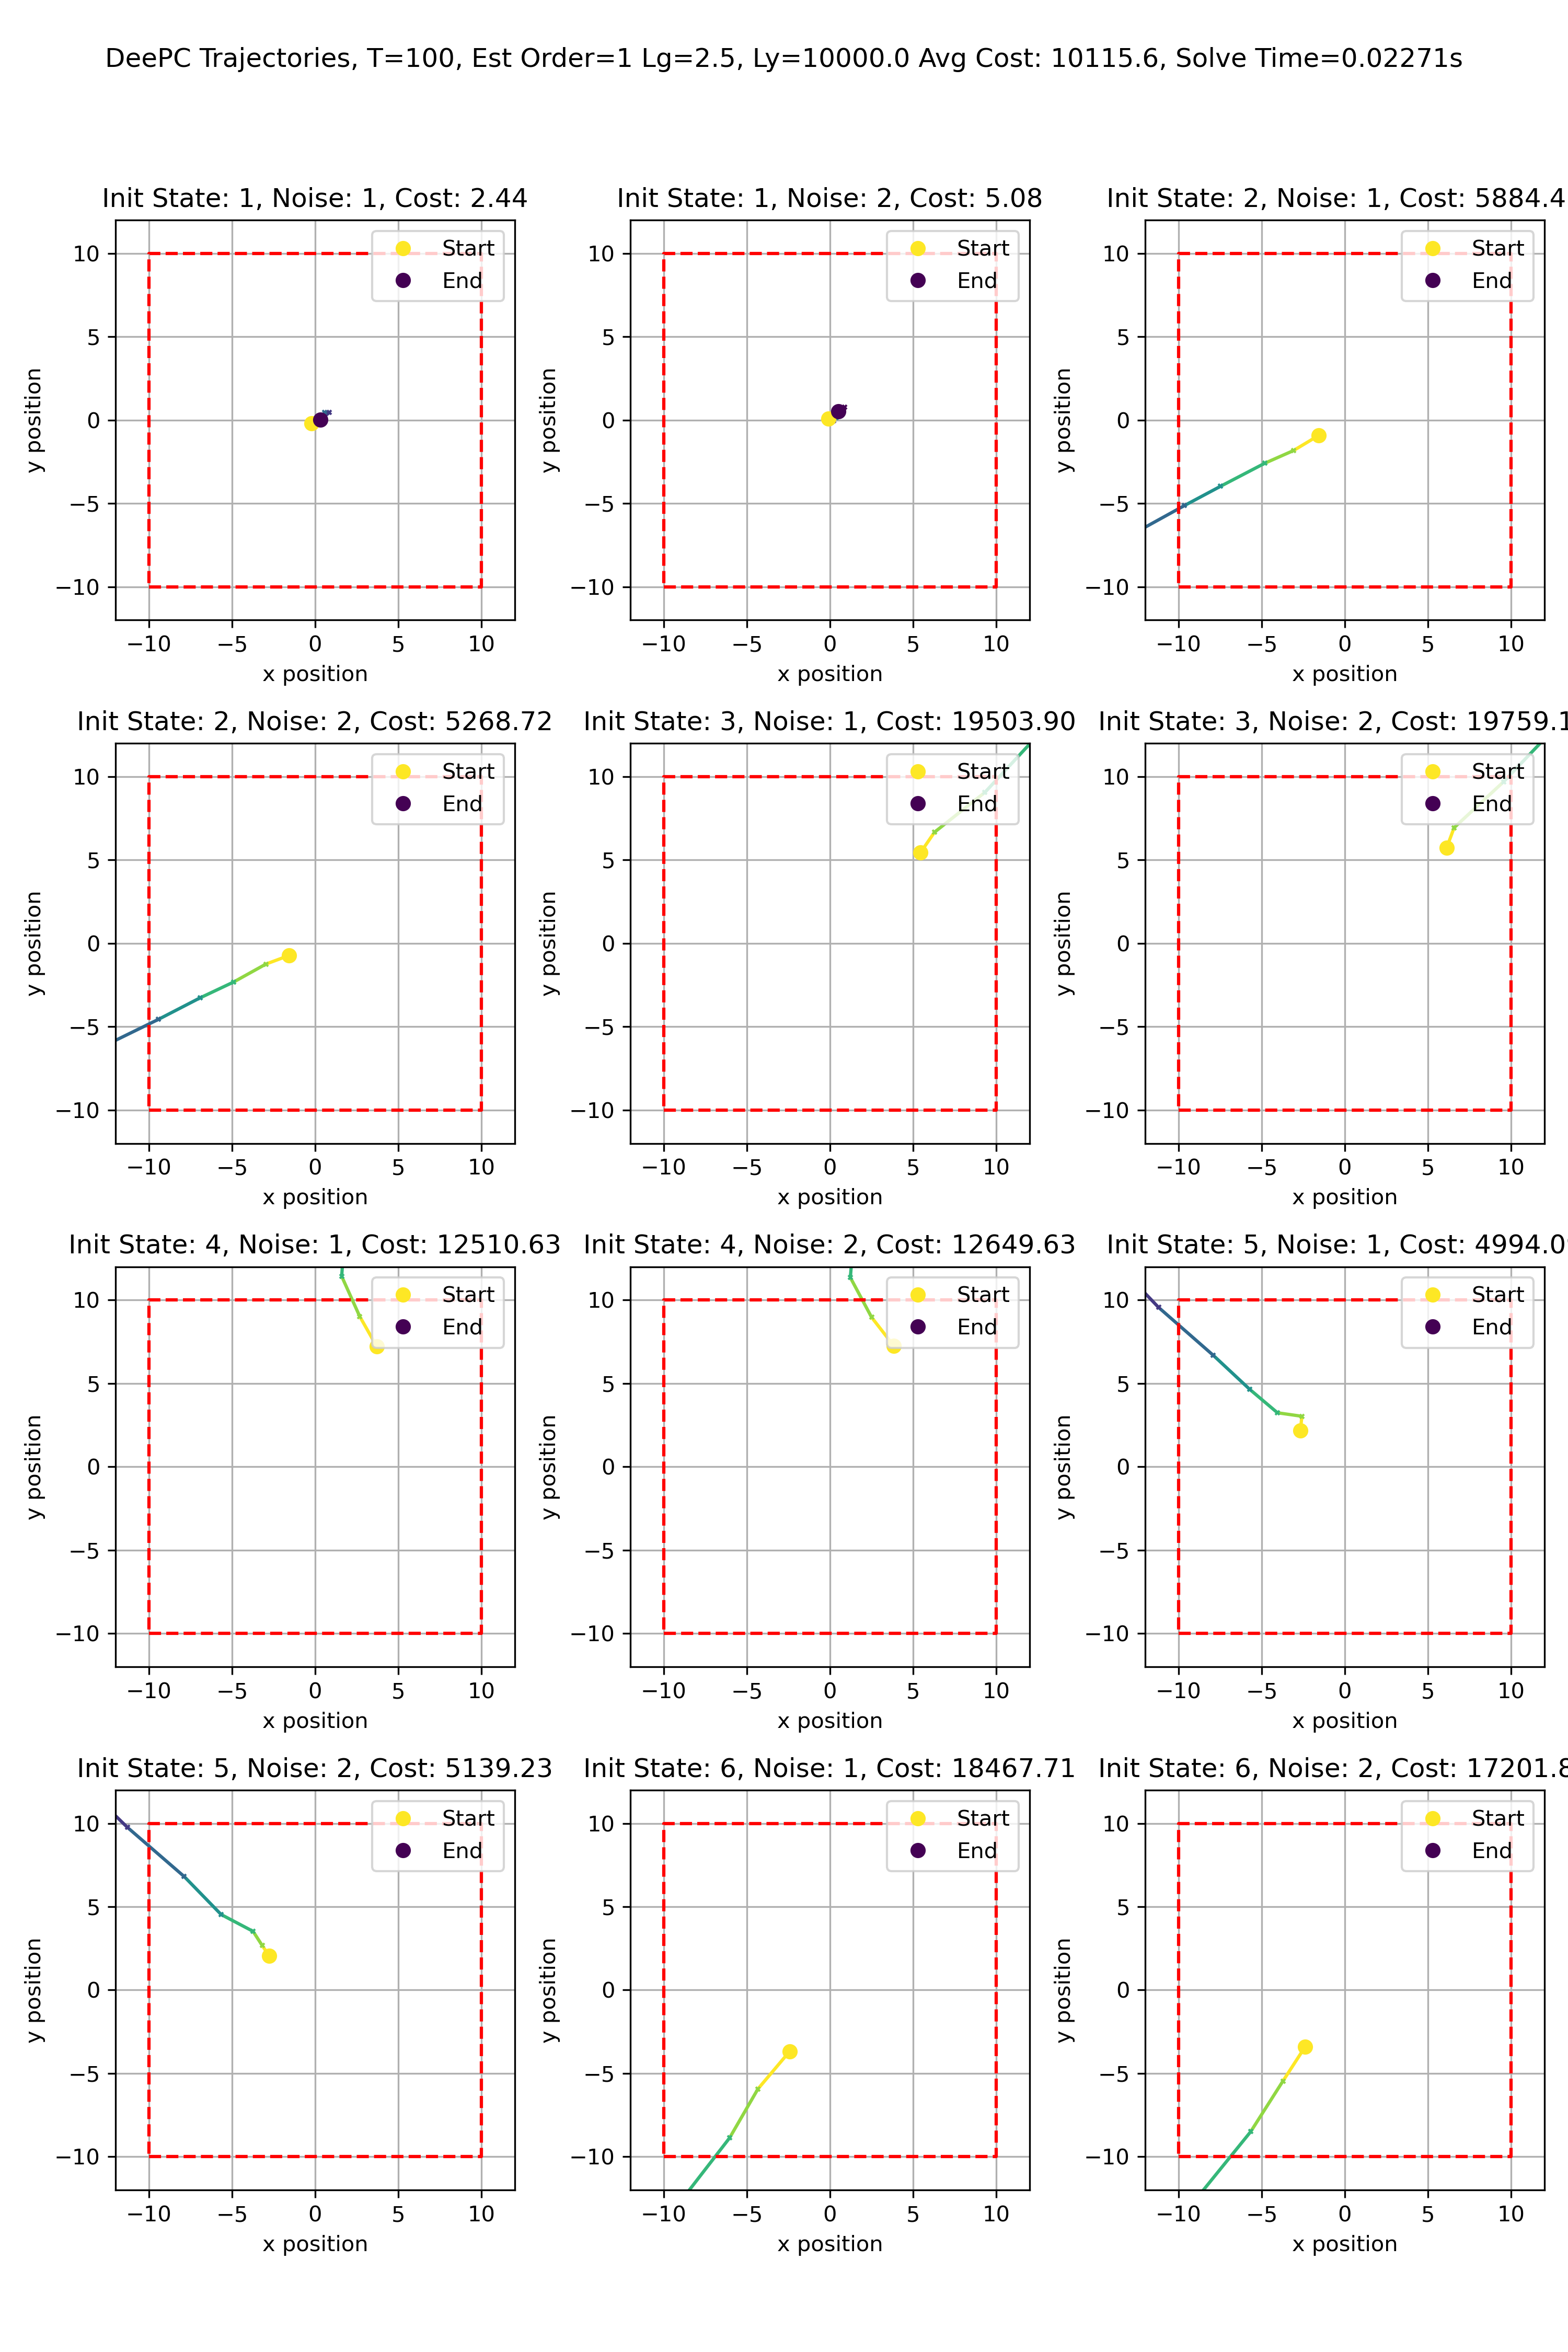
\includegraphics[width=0.85\linewidth]{./figures/DeePC_trajectories_100_1_2.5_10000.0.png}
    \caption{$\lambda_g=2.5, \lambda_y=1\mathrm{e}4, \text{order}=1, T=100$ Completely collapses, since there is not enough data}
    \label{fig:enter-label}
\end{figure}

% Sligthly Over estimate order
\begin{figure}
    \centering
    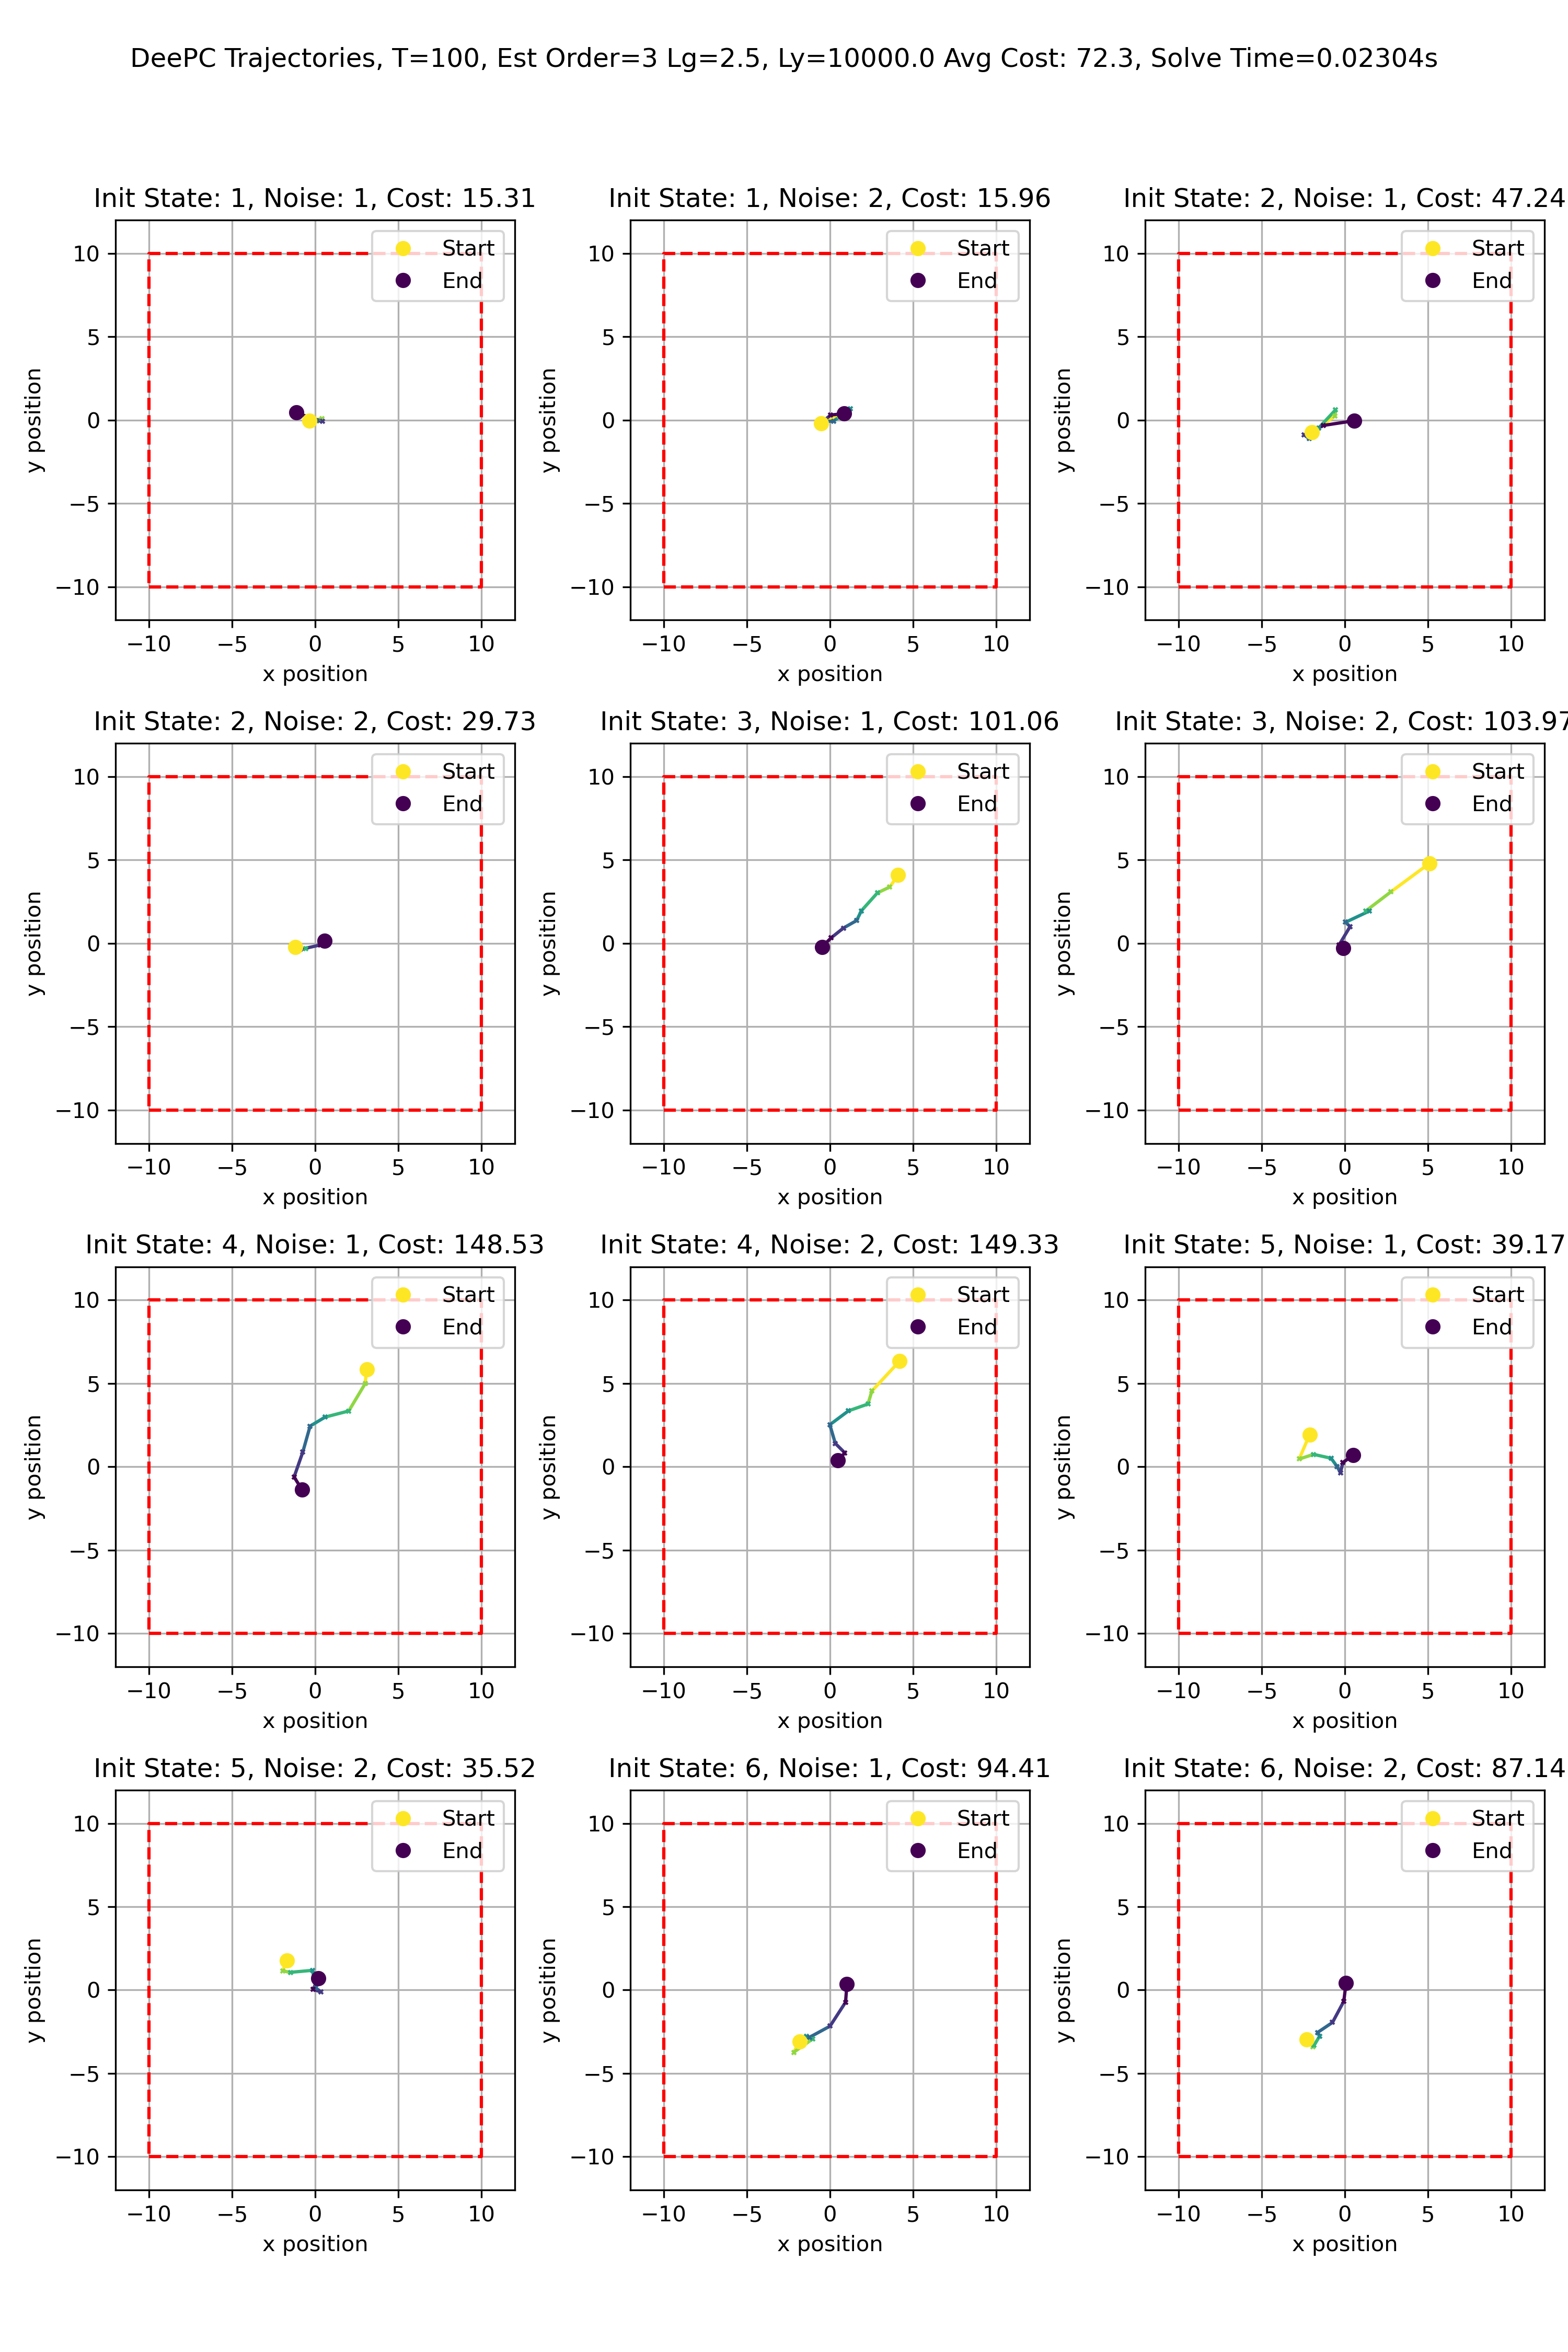
\includegraphics[width=0.85\linewidth]{./figures/DeePC_trajectories_100_3_2.5_10000.0.png}
    \caption{$\lambda_g=2.5, \lambda_y=1\mathrm{e}4, \text{order}=3, T=100$ Sligthly over estimating the order does not cause issues}
    \label{fig:enter-label}
\end{figure}

% Using less data
\begin{figure}
    \centering
    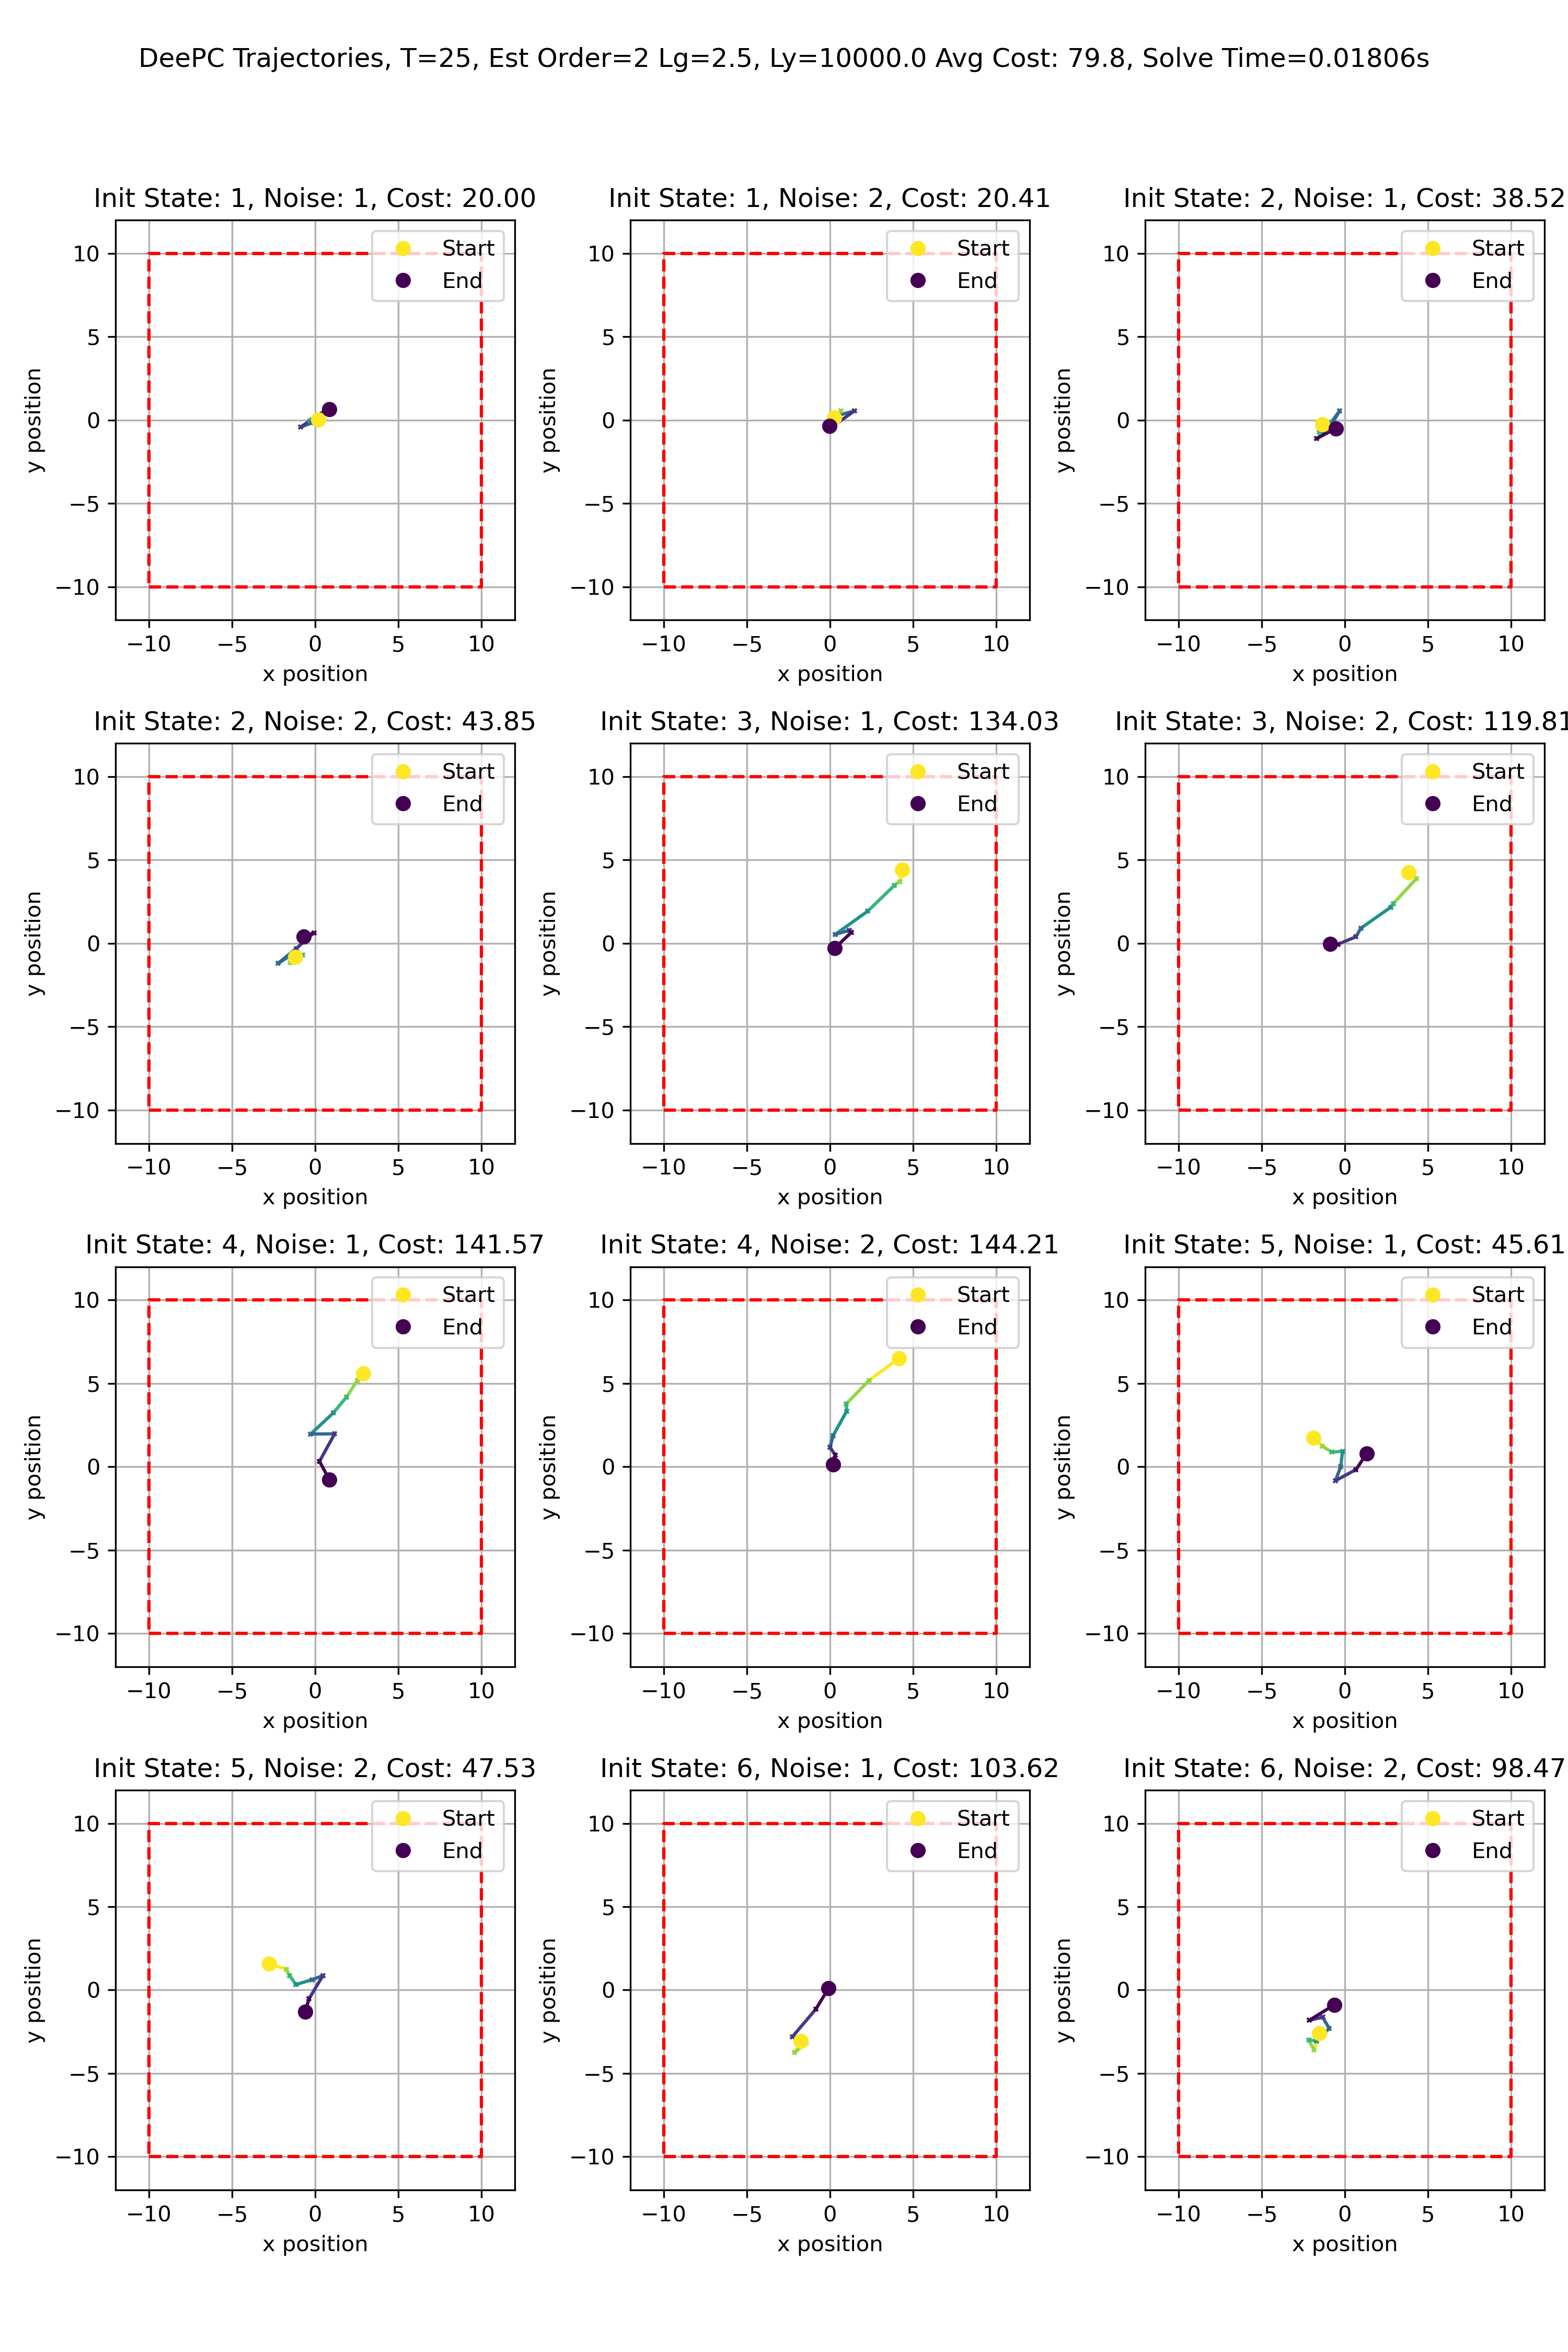
\includegraphics[width=0.85\linewidth]{./figures/DeePC_trajectories_25_2_2.5_10000.0.png}
    \caption{$\lambda_g=2.5, \lambda_y=1\mathrm{e}4, \text{order}=2, T=25$ Performs fairly well, since it is a linear system, we do not actually need too much data}
    \label{fig:enter-label}
\end{figure}

% Do not regulate the model size
\begin{figure}
    \centering
    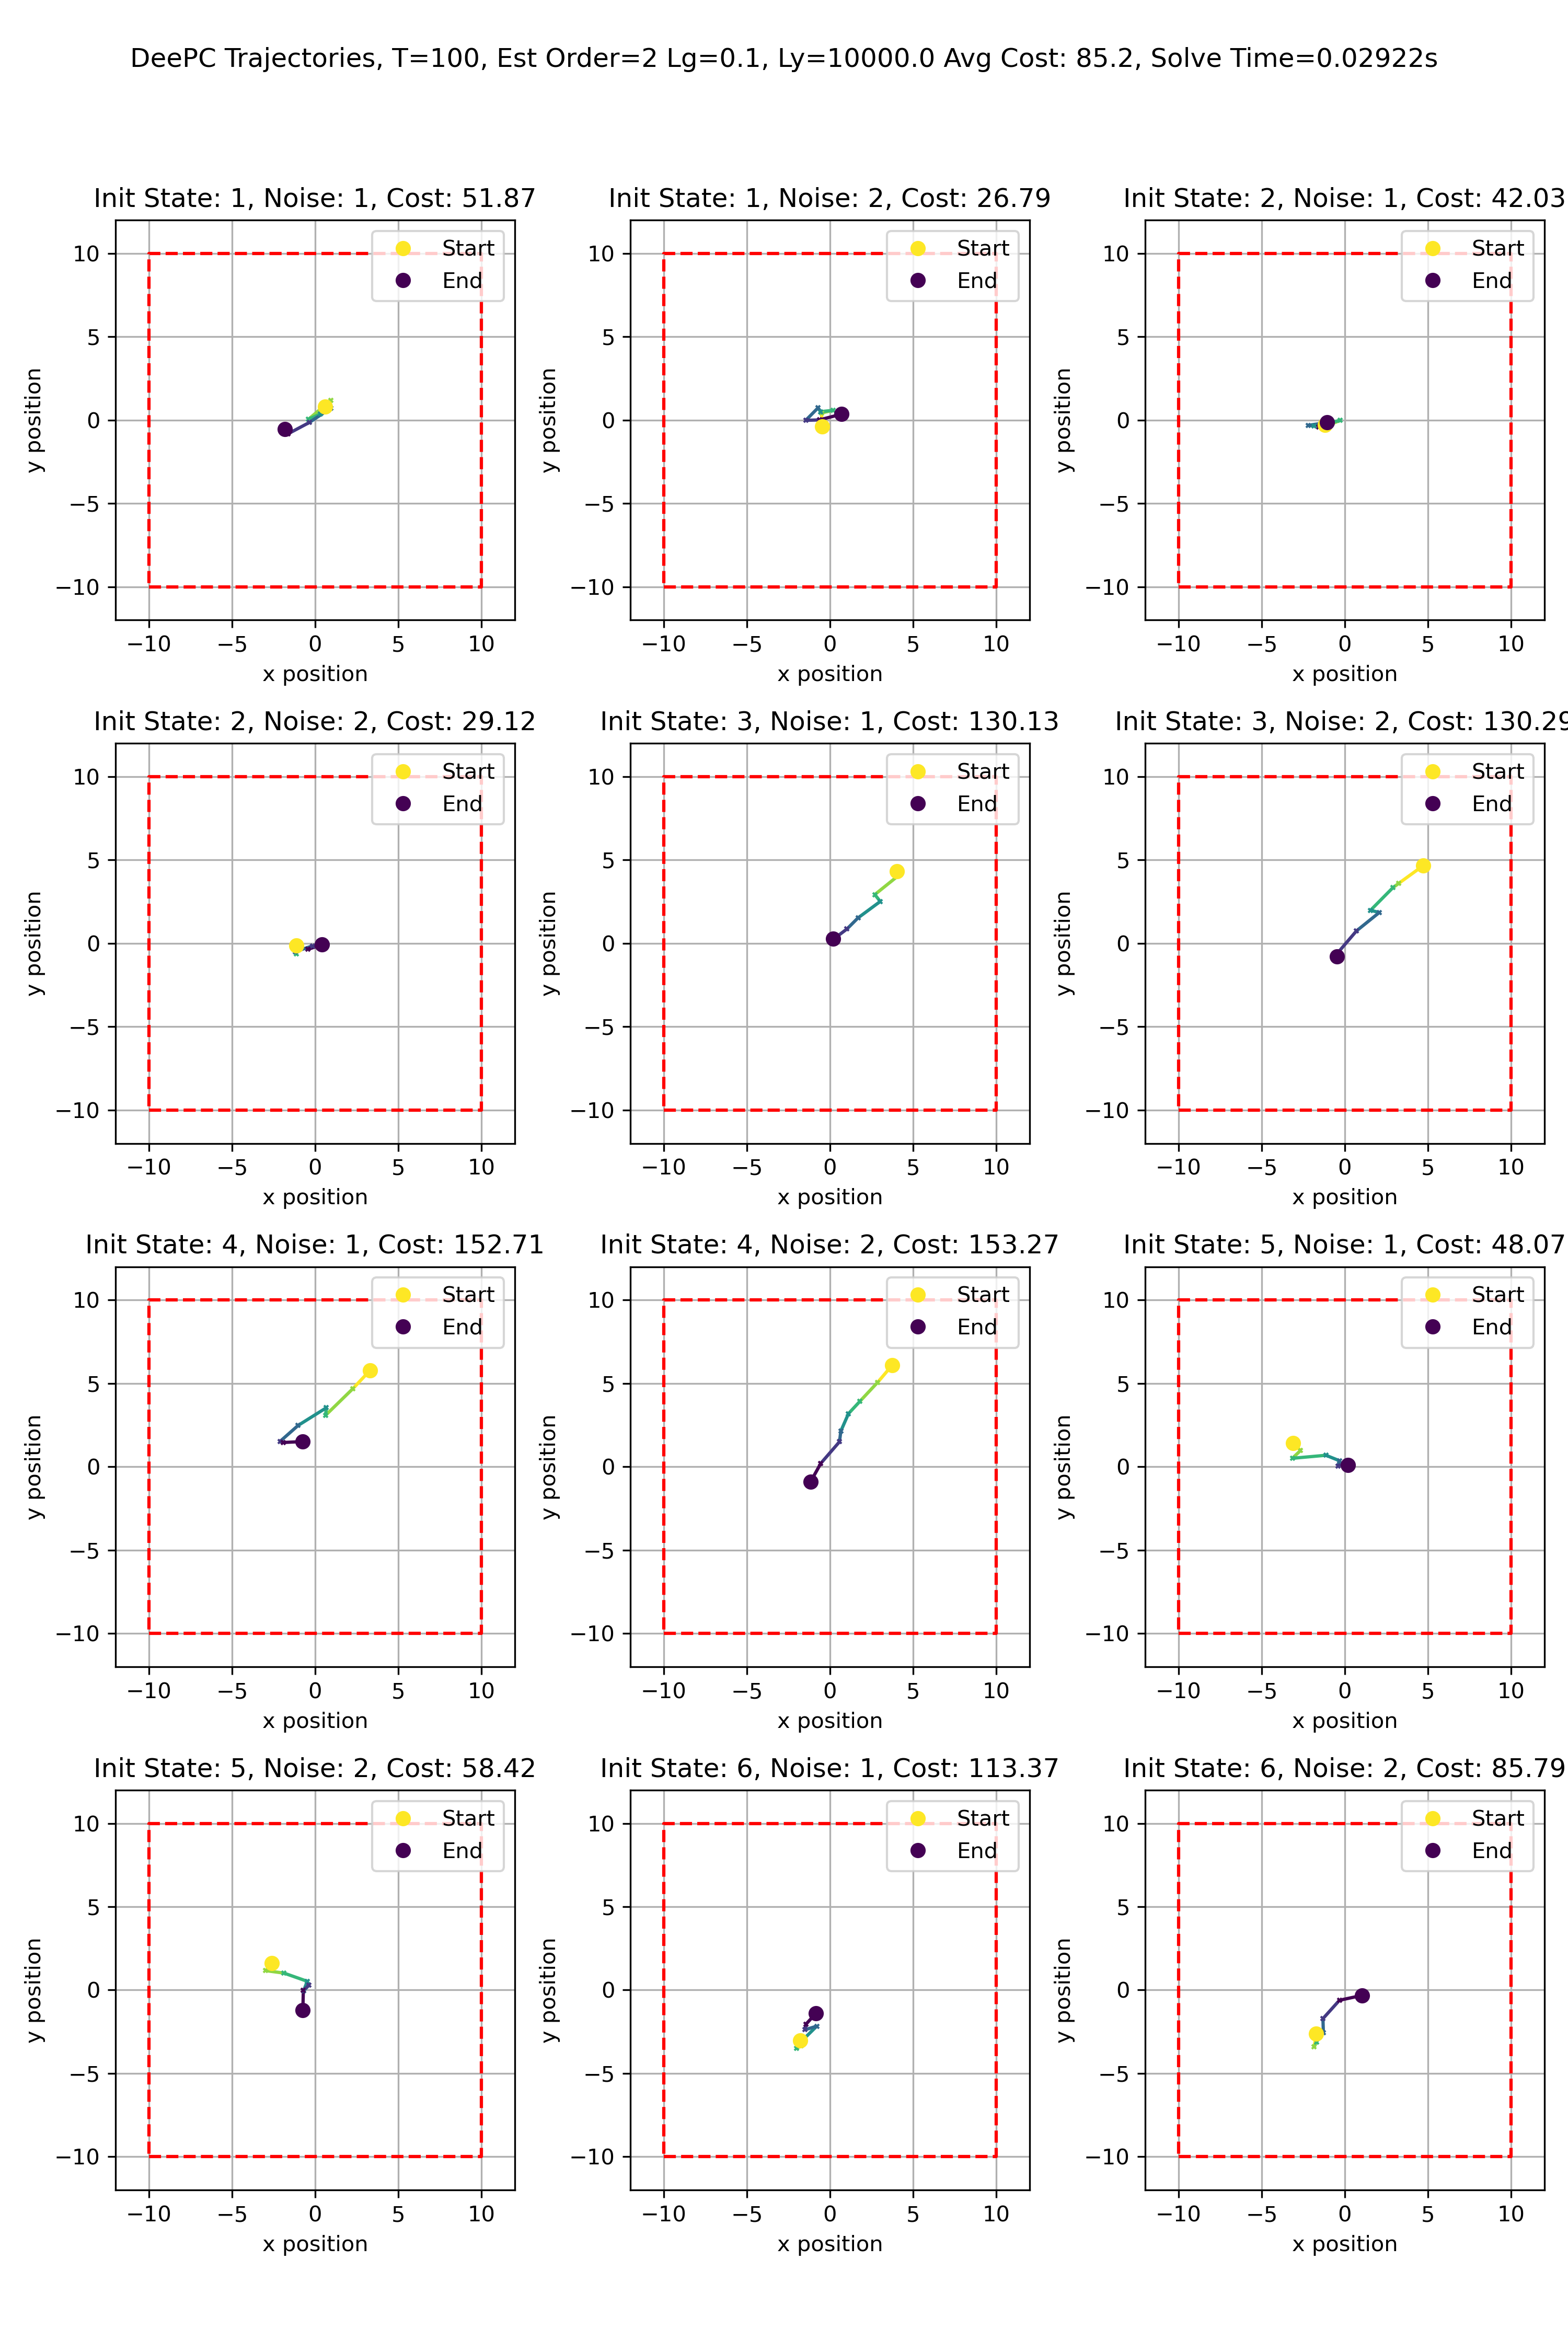
\includegraphics[width=0.85\linewidth]{./figures/DeePC_trajectories_100_2_0.1_10000.0.png}
    \caption{$\lambda_g=0.1, \lambda_y=1\mathrm{e}4, \text{order}=2, T=100$ Since it is a linear system you do not need to regulate the model size too much.}
    \label{fig:enter-label}
\end{figure}


% Heavily regulate the model size
\begin{figure}
    \centering
    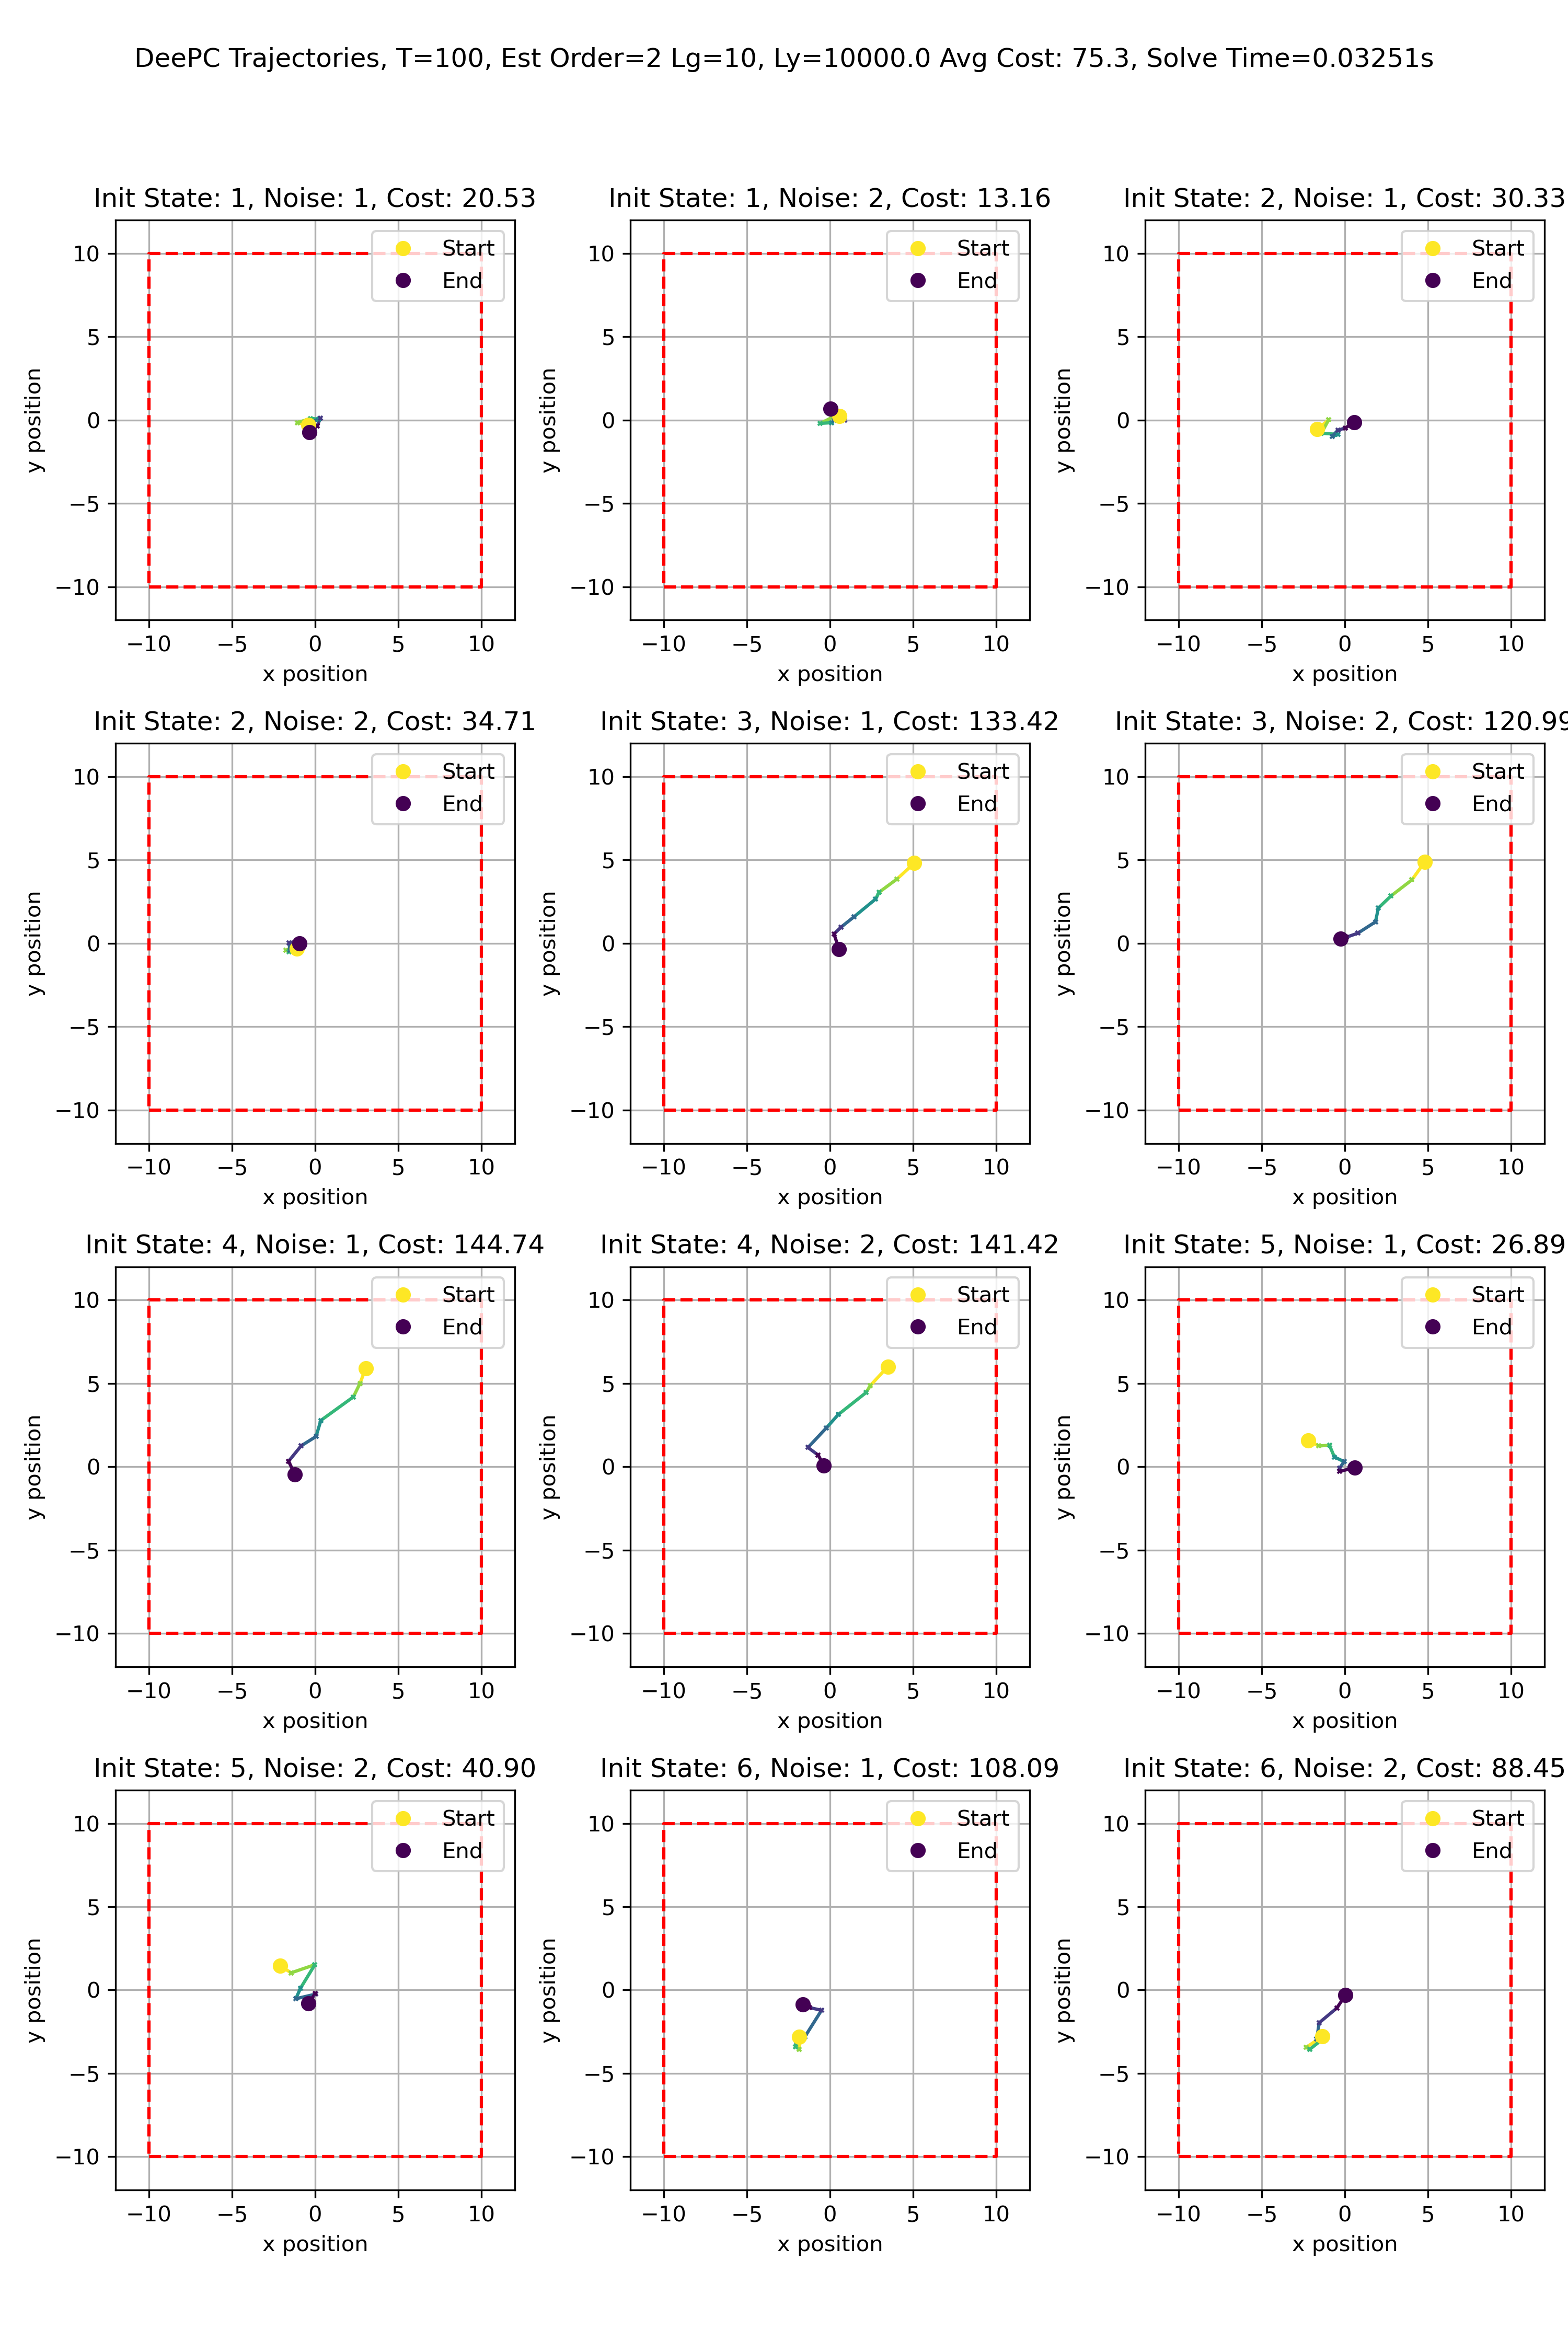
\includegraphics[width=0.85\linewidth]{./figures/DeePC_trajectories_100_2_10_10000.0.png}
    \caption{$\lambda_g=10, \lambda_y=1\mathrm{e}4, \text{order}=2, T=25$ Heavily regulating the model size leads to adverse performance.}
    \label{fig:enter-label}
\end{figure}


% Heavily regulate model give
\begin{figure}
    \centering
    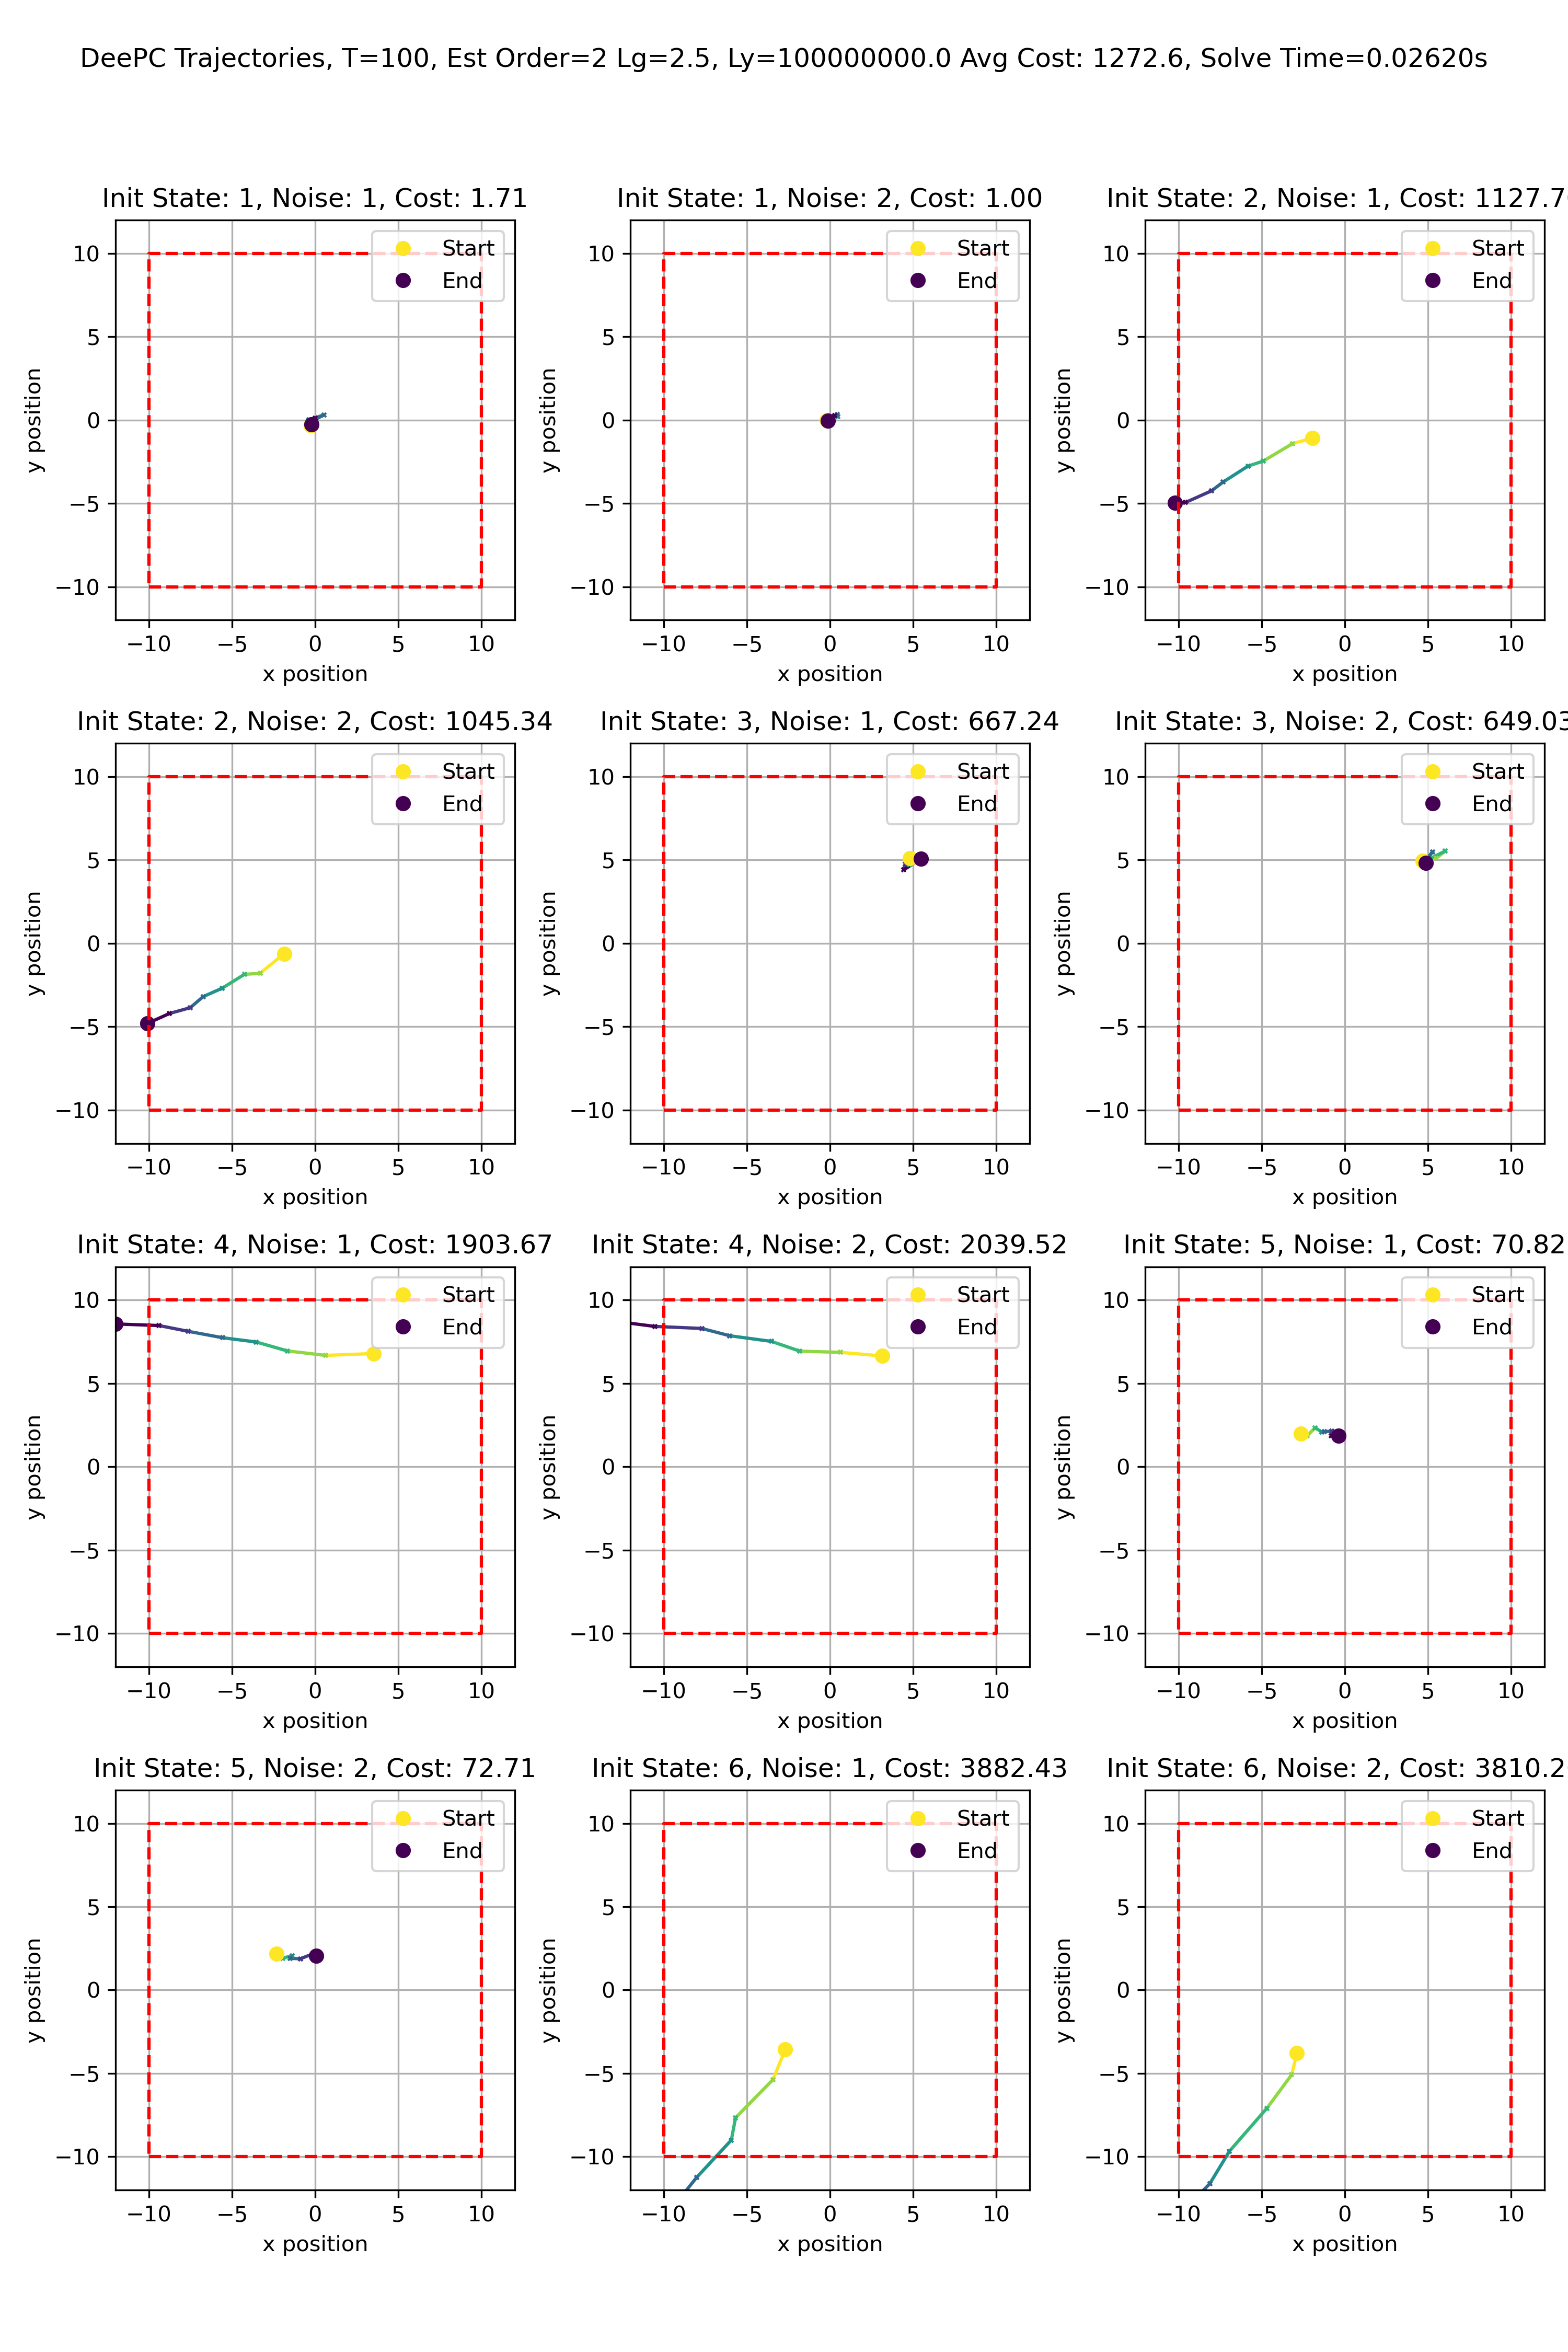
\includegraphics[width=0.85\linewidth]{./figures/DeePC_trajectories_100_2_2.5_100000000.0.png}
    \caption{$\lambda_g=2.5, \lambda_y=1\mathrm{e}8, \text{order}=2, T=25$ Heavily regulating the model size leads to adverse performance.}
    \label{fig:enter-label}
\end{figure}


Other tests not mentioned:
These tests dailed to converge:
\begin{itemize}
    \item Heavily Over Estimating the Order: Using order = 10 completely failed.
    \item Under Regulating the Give: Without regulating the give, the value of sigma grows extremely high leading the model to be meaningless.
\end{itemize}




The following trends were observed
\begin{itemize}
    \item \textbf{Order Estimate}: It is a good rule of thumb to match the correct estimate or go sligthly above. If it fails then decrease the estimate order
    \item \textbf{T}: For a linear system more or less data does not affect performance too much
    \item \( \mathbf{\lambda_g} \): This did not affect the performance for the linear system, but this would be important for noisy data collection/ a non linear system
    \item \( \mathbf{\lambda_y} \): This is really important to keep high so that the model is actually constrained
\end{itemize}
\subsection{Constraint Satisfaction}
DeePC respected all input and state box constraints after the initial alignment phase, since the constraints are embedded within the optimization problem. Some constraint violations occured when the implicit model \(g\) did not well represent the model for some hyperparameters and during the offline data collection period.

\subsection{Extension: Speeding up DeePC}
The offline data collection leaves a lot of redundancy in the Hankel matrix, which leads to slow solve times. This can be fixed by using a Low Rank Approximation of the Hankel Matricies. This is done with SVD, and taking the full rank of the Hankel Matrix rather than an overdetermined system.

On average this computes trajectories over 50\% faster for large datasets($T>500$), without any noticable performance decrease.

\begin{figure}
    \centering
    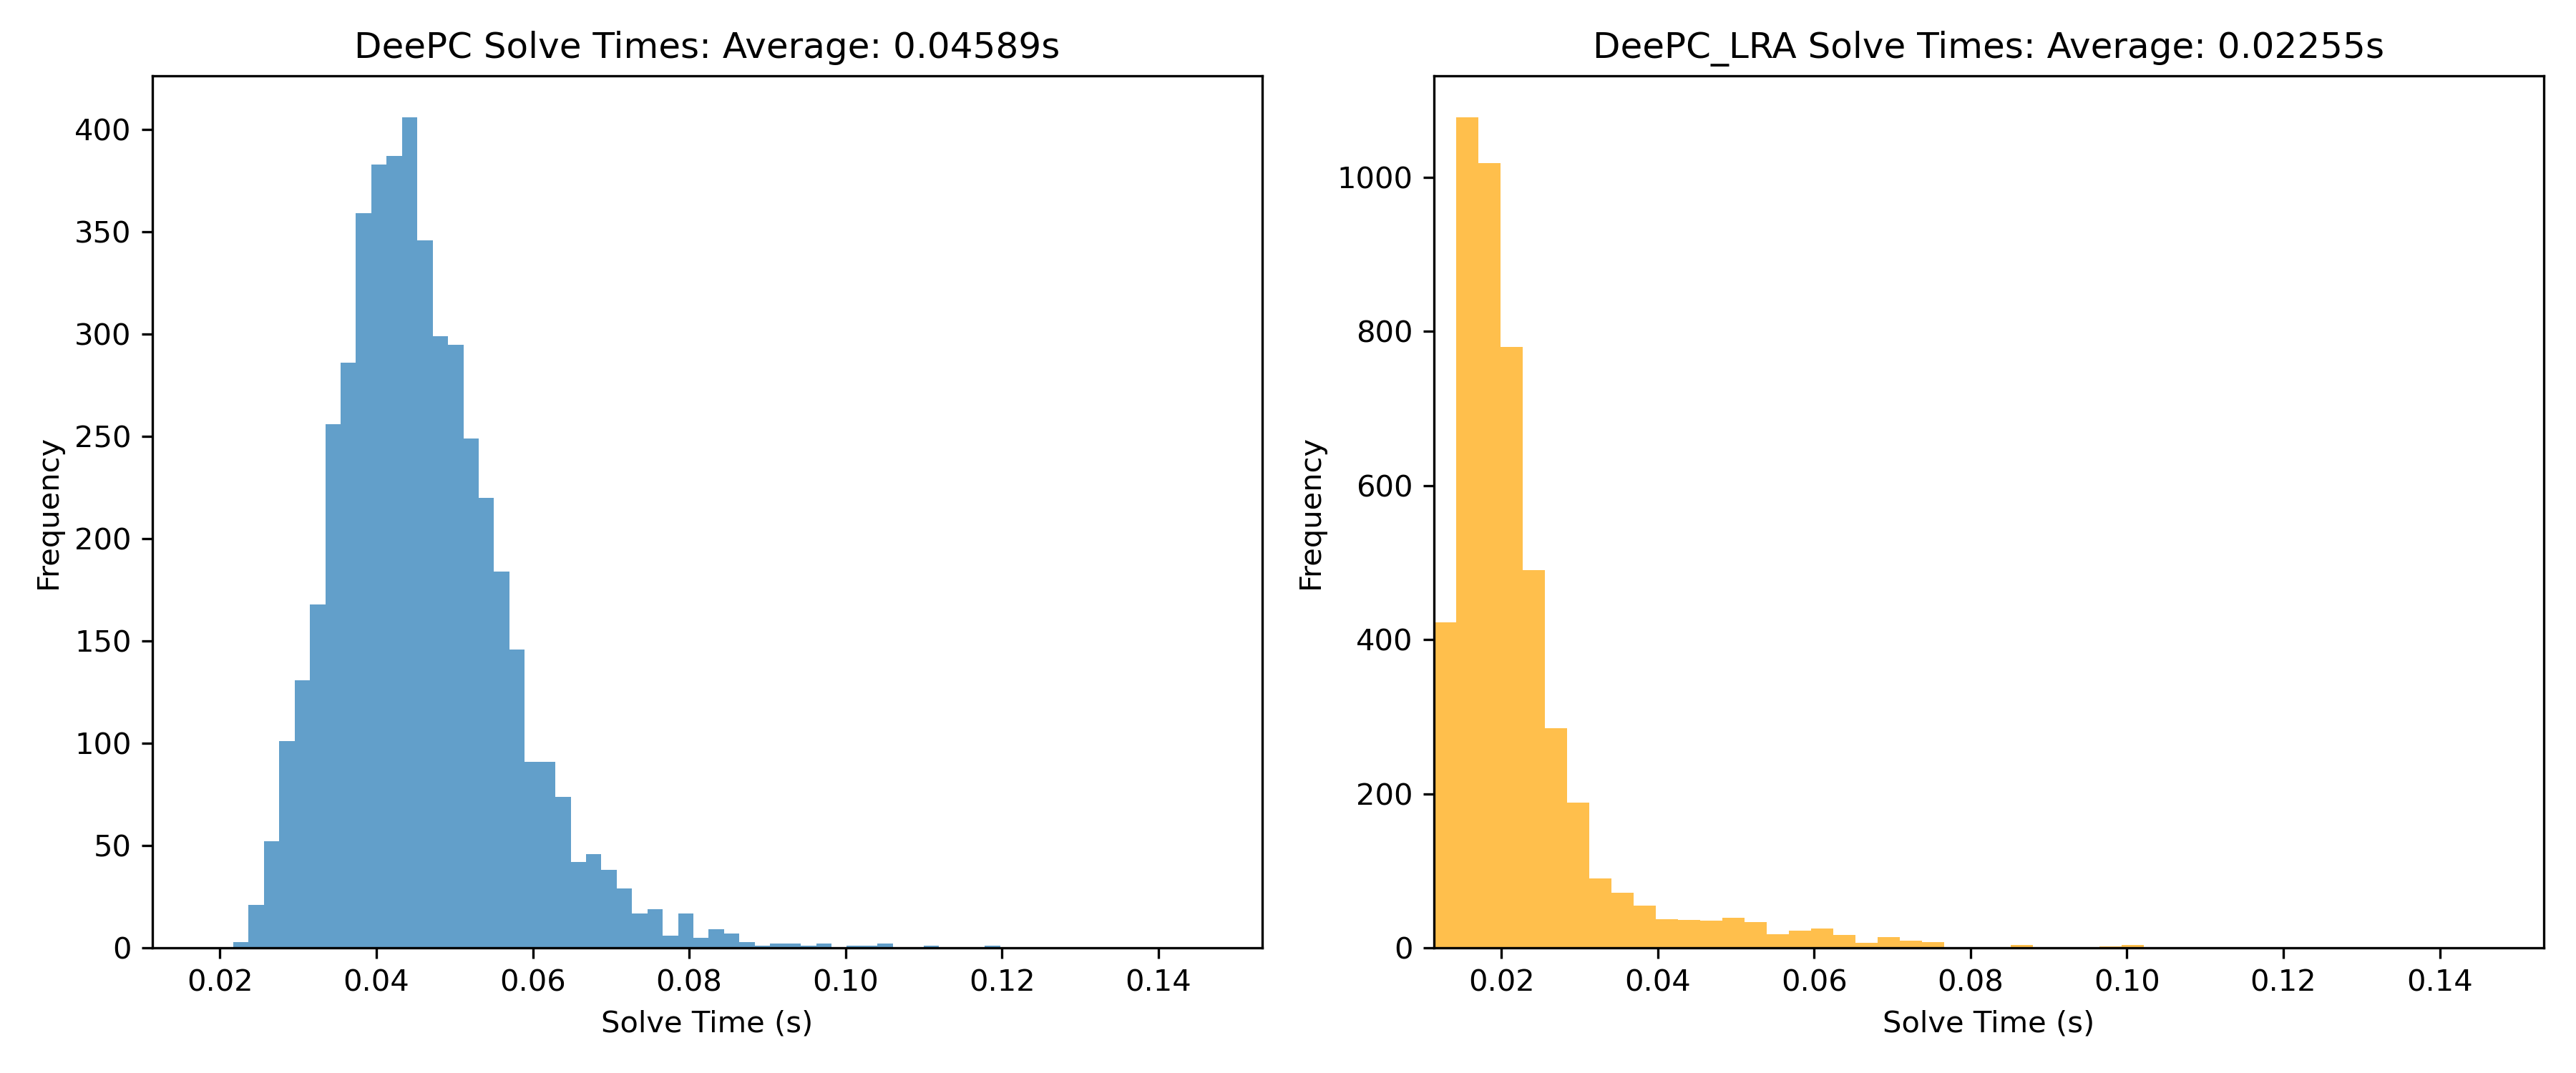
\includegraphics[width=0.85\linewidth]{./figures/deePC_solve_times.png}
    \caption{Solve Times using and not using a low rank approximation}
    \label{fig:enter-label}
\end{figure}

Using a Low Rank Approximation speeds up the DeePC solver over 50\% in the above tests. However there are two important notes to make:

Performance highly depends on the "rank" of the system. It is significantly easier to speed up a linear system than a system with a complex behavior, since the linear system has a low rank.

Collecting more data will slow down a normal DeePC controller by a fair bit, since the implicit dynamics model is a lot larger. It will not significantly slow down the low rank DeePC controller, since the SVD will reduce the dimensionality of the Hankel matrix. The only downside is that the SVD computation is expensive, but it can be done offline unless the horizon is changing frequently.

Collecting more data helps the DeePC controller to better approximate the system dynamics, and the Low Rank Controller allows you to collect more data without significantly slowing down the controller.


\section{Takeaways}
Since this was a data driven method, the biggest takeaways were 


\begin{itemize}
    \item \textbf{Data heavily impacts performance.}  
    DeePC requires persistent excitation, along with varied and rich data to construct a representative implicit model.

    \item \textbf{Hyperparameter tuning is non-trivial.}  
    Regularization parameters (\( \lambda_g, \lambda_y \)) and window sizes (\(T_{\text{ini}}, N\)) significantly affect performance. This means that empirical tuning is required for DeePC to perform.

    \item \textbf{DeePC is slow for large datasets} However using a low rank approximation can significantly speed up this time.
\end{itemize}

\subsection*{Future Work}
One of the most interesting extensions would be to extend DeePC to nonlinear systems. Attempting to do this on a pendulum requires quite a lot of hyperparameter tuning, wich is why it is not in this report.
The other interesting extension, would be to explore the low rank approximation further, since using the rank as a hyperparameter can significantly speed up the DeePC controller, and allow it to scale to larger datasets. At the same time, this may be challenging since underestimating the rank can lead to failure.
\section{Appendix}
Code is released on \href{https://github.com/Sanjit1/DeePC}{github}. 


\href{https://arxiv.org/abs/1811.05890#}{Data-Enabled Predictive Control on Arxiv}

\href{https://docs.google.com/presentation/d/1G0WMO9AojQ1DTrTkCCZOjw6U850QCCY_Jp0nHHJWcT4/edit?usp=sharing}{My slides on the material}
\end{document}
